% !TEX TS-program = pdflatex
% !TEX encoding = UTF-8 Unicode

% This is a simple template for a LaTeX document using the "article" class.
% See "book", "report", "letter" for other types of document.

\documentclass[8pt]{article} % use larger type; default would be 10pt

\usepackage[utf8]{inputenc} % set input encoding (not needed with XeLaTeX)
\usepackage{bchart}
\usepackage{longtable}
\usepackage{pgfgantt}
\usepackage{calendar} % Use the calendar.sty style
\usepackage{calc}
\usepackage{ifthen}
\usepackage{tkz-base}
\usepackage{pdfpages}
\usepackage{hyperref}
\usepackage{pgfplots}
\usepackage{tkz-kiviat,numprint,fullpage} 
\usepackage{pgfplotstable} 
\usetikzlibrary{arrows}
\usepackage{paralist} % very flexible & customisable lists (eg. enumerate/itemize, etc.)
\usepackage{dcolumn}
\usepackage{booktabs}
\usepackage{lscape}
\usepackage{pgf-pie}
\usepackage{verbatim}
\usepackage{animate}
\usepackage{sfmath}
\usepackage{listings}
\usepackage{xcolor}

\definecolor{codegreen}{rgb}{1,0,0}
\definecolor{codegray}{rgb}{0.5,0.5,0.5}
\definecolor{codepurple}{rgb}{0.58,0,0.82}
\definecolor{backcolour}{rgb}{0.95,0.95,0.92}

%%% Examples of Article customizations
% These packages are optional, depending whether you want the features they provide.
% See the LaTeX Companion or other references for full information.

\usepackage{textcomp}
%\usepackage{hyperref}

%%% PAGE DIMENSIONS
\usepackage{geometry} % to change the page dimensions
\geometry{a4paper} % or letterpaper (US) or a5paper or....
% \geometry{margin=2in} % for example, change the margins to 2 inches all round
% \geometry{landscape} % set up the page for landscape
%   read geometry.pdf for detailed page layout information

\usepackage{graphicx} % support the \includegraphics command and options

% \usepackage[parfill]{parskip} % Activate to begin paragraphs with an empty line rather than an indent

%%% PACKAGES
\usepackage{booktabs} % for much better looking tables
\usepackage{array} % for better arrays (eg matrices) in maths
\usepackage{paralist} % very flexible & customisable lists (eg. enumerate/itemize, etc.)
\usepackage{verbatim} % adds environment for commenting out blocks of text & for better verbatim
\usepackage{subfig} % make it possible to include more than one captioned figure/table in a single float
% These packages are all incorporated in the memoir class to one degree or another...

%%% HEADERS & FOOTERS
\usepackage{fancyhdr} % This should be set AFTER setting up the page geometry
\pagestyle{fancy} % options: empty , plain , fancy
\renewcommand{\headrulewidth}{0pt} % customise the layout...
\lhead{}\chead{}\rhead{}
\lfoot{}\cfoot{\thepage}\rfoot{}

%%% SECTION TITLE APPEARANCE
\usepackage{sectsty}
\allsectionsfont{\sffamily\mdseries\upshape} % (See the fntguide.pdf for font help)
% (This matches ConTeXt defaults)

%%% ToC (table of contents) APPEARANCE
\usepackage[nottoc,notlof,notlot]{tocbibind} % Put the bibliography in the ToC
\usepackage[titles,subfigure]{tocloft} % Alter the style of the Table of Contents
\renewcommand{\cftsecfont}{\rmfamily\mdseries\upshape}
\renewcommand{\cftsecpagefont}{\rmfamily\mdseries\upshape} % No bold!

%%% END Article customizations

%%% The "real" document content comes below...

%\includegraphics[width=.2\textwidth]{Logo.png}

\title{Finance}
\author{\copyright Frederic Kerdraon}
%\date{} % Activate to display a given date or no date (if empty),
         % otherwise the current date is printed 


%\addtobeamertemplate{frametitle}{}{%
%\begin{tikzpicture}[remember picture,overlay]
%\node[anchor=north west,yshift=2pt] at (current page.north west) {\includegraphics[height=0.8cm]{Logo1}};
%\end{tikzpicture}}

\begin{document}
\maketitle
\hspace*{-1cm}\includegraphics[width=.2\textwidth,left]{Logo.png}
%//FK - Here we have a problem
{\footnotesize
Data are aggregated between Initial date: \textbf{2000-01-01} and Last date: \textbf{2018-11-16 00:00:00}

}
\tableofcontents

%FK - There is no need for an introduction
%\section{Introduction}

%This document summurizes all the important informations necessary to facilitate things and remove a lot of stress. It's been put together thanks to \LaTeX. This is designed to help make optimal decisions for a not so short lifetime.

{\footnotesize
%Ce n'est pas parceque les choses sont difficiles que nous n'osons pas, c'est parceque nous n'osons pas qu'elles sont difficiles.
}
%\makebox[2\width]{hello}

\newcounter{a}
\newcounter{b}
%----------------------------------------------------------
\newcommand{\slice}[4]{
  \pgfmathparse{0.5*#1+0.5*#2}
  \let\midangle\pgfmathresult

   slice
  \draw[thick,fill=black!10] (0,0) -- (#1:1) arc (#1:#2:1) -- cycle;

   outer label
  \node[label=\midangle:#4] at (\midangle:1) {};

   inner label
  \pgfmathparse{min((#2-#1-10)/110*(-0.3),0)}
  \let\temp\pgfmathresult
  \pgfmathparse{max(\temp,-0.5) + 0.9}
  \let\innerpos\pgfmathresult
  \node at (\midangle:\innerpos) {#3};
}

\lstdefinestyle{mystyle}{
    backgroundcolor=\color{backcolour},
    commentstyle=\color{codegreen},
    keywordstyle=\color{magenta},
    numberstyle=\tiny\color{codegray},
    stringstyle=\color{codepurple},
    basicstyle=\ttfamily\footnotesize,
    breakatwhitespace=false,
    breaklines=true,
    captionpos=b,
    keepspaces=true,
    numbers=left,
    numbersep=5pt,
    showspaces=false,
    showstringspaces=false,
    showtabs=false,
    tabsize=2
}

\lstset{style=mystyle}

\section{Management summary}

\subsection{PnL Projections}

%Le nombre de simulations est egal au nombre d'arrangements des targets\\
%Pour 8 target, il devrait y avoir un 8! scenarios\\
%Les scenarios sont ordonnes par facilite de mise en oeuvre min(complexity, cost,etc)\\

\subsubsection{Latex Graph of the scenarios}

Initial parameters for the simulations.\\

%\begin{itemize}
%	\item {\$TotalDrift}
%	\item {\$TotalScenTox}
%	\item {\$TotalScenDebt}
%	\item {\$TotalScenCash}
%	\item {\$TotalScenToxDebt}
%	\item {\$TotalScen = 0}
%\end{itemize}

We apply the scenarios below to see what we get after a few iterations\\

%\begin{itemize}
%	\item {\$Scen}
%	\item {\$Scenario reduction of Toxics by 231}
%	\item {\$Scenario reduction of the Debt by 529*0.4}
%	\item {\$Scenario reduction of the Cash by 755*.5}
%	\item {\$Scenario reduction of the Toxics and Debt by 231+529*.4}
%\end{itemize}

my @Scen = (231,529*.4,755*.5,231+529*.4,1000,700,800,950,750);\\

\begin{itemize}
	\item{The first simulation apply a reduction of the Toxics by 231 euros each month}
	\item{The second scenario apply a reduction of the debt by 40 percent of the 529}
	\item{The third one divide the amount of cash spent by 50 percent}
	\item{The fourth one cumulate the reduction of the toxics by 231 euros with the amount of cash spent reduced by 50 percent}
	\item{The fifth one is a reduction of 1000 euros each month}
	\item{The sifth one is a reduction of 700 euros each month}
	\item{The seventh one is a reduction of 800 euros each month}
	\item{The eighth one is a reduction of 950 euros each month}
	\item{The nineth one is a reduction of 750 euros each month}
\end{itemize}

On the graph we can notice that all the scenarios are positive, as they were built to show how to maximize profit, just by managing the charge, and especially useless charges.\\

%my $Drift = $row->{Drift};
%$NewDrift = $Drift + $NewDrift;
%my $KDrift = $Drift/$Unit;
%$TotalDrift = $TotalDrift + $Drift;
%$TotalScenTox = $TotalDrift + $ScenToxics*$Count;
%$TotalScenDebt = $TotalDrift + $ScenDebt*$Count;
%$TotalScenCash = $TotalDrift + $ScenCash*$Count;
%$TotalScenToxDebt = $TotalDrift + $ScenToxDebt*$Count;

%//FK - Here we have a pb

%Dimensions too large....
This graph is dependant on: \$NUM\_RECORDS\_BALANCE which was set to 1000. When we set it to 10 it works. It's ugly, but it works.\\

We would need to input all the data into the database and read it through Scilab to get a proper graph.
%\setlength{\unitlength}{1cm}
\begin{picture}(12,11)(0,0)
\put(0,0){\vector(1,0){12.1}}
\put(12,-.35){$Month$}
\put(0,-6){\vector(0,1){12}}
\put(0,6.5){\makebox(0,0){$PnL$)}}
\put( -0.5,1){$1$}
\put( -0.5,2){$2$}
\put( -0.5,3){$3$}
\put( -0.5,4){$4$}
\put( -0.5,5){$5$}
\put( -0.5,6){$6$}
\put( -0.5,-1){$-1$}
\put( -0.5,-2){$-2$}
\put( -0.5,-3){$-3$}
\put( -0.5,-4){$-4$}
\put( -0.5,-5){$-5$}
\put( -0.5,-6){$-6$}
\qbezier(0.0,0.0)(1.2384,0.0)(2.0,2.7622)
\linethickness{.090mm}
\put( 0,6){$1$}
\put( 0,0.472810){\line(2,0){.2}}
\put( 0,0){\line(0,1){0.472810}}
\put( 0.2,0){\line(0,1){0.472810}}
\put( 0,0.572810){$Scen0$}
\put( 0,0.703810){\line(2,0){.5}}
\put( 0,0){\line(0,1){0.703810}}
\put( 0.5,0){\line(0,1){0.703810}}
\put( 0,0.684410){\line(2,0){.5}}
\put( 0,0){\line(0,1){0.684410}}
\put( 0.5,0){\line(0,1){0.684410}}
\put( 1,6){$2$}
\put( 1,-0.002590){\line(2,0){.2}}
\put( 1,-0.002590){\line(0,1){0.002590}}
\put( 1.2,-0.002590){\line(0,1){0.002590}}
\put( 1,-0.302590){$Scen0$}
\put( 1,0.459410){\line(2,0){.5}}
\put( 1,0){\line(0,1){0.459410}}
\put( 1.5,0){\line(0,1){0.459410}}
\put( 1,0.420610){\line(2,0){.5}}
\put( 1,0){\line(0,1){0.420610}}
\put( 1.5,0){\line(0,1){0.420610}}
\end{picture}


%This one works but gives a huge table
%The scenarios given in the table are only examples, the real scenarios are provided in the graph below
\begin{longtable}{|c|c|c|c|c|c|}
\hline
\multicolumn{6}{|c|}{Scenarios} \\
\hline
PnL; CumPnL; Tox; Debt(40%); Cash(50%); Tox-Debt(40%)
PnL & CumPnL & Tox & Debt(40\%) & Cash(50\%) & Tox-Debt(40\%)
\hline
472;472;703;684;850;915
472 & 472 & 703 & 684 & 850 & 915\\
\hline
-475;-2;459;420;752;882
-475 & -2 & 459 & 420 & 752 & 882\\
\hline
\end{longtable}


\subsubsection{Barplot}

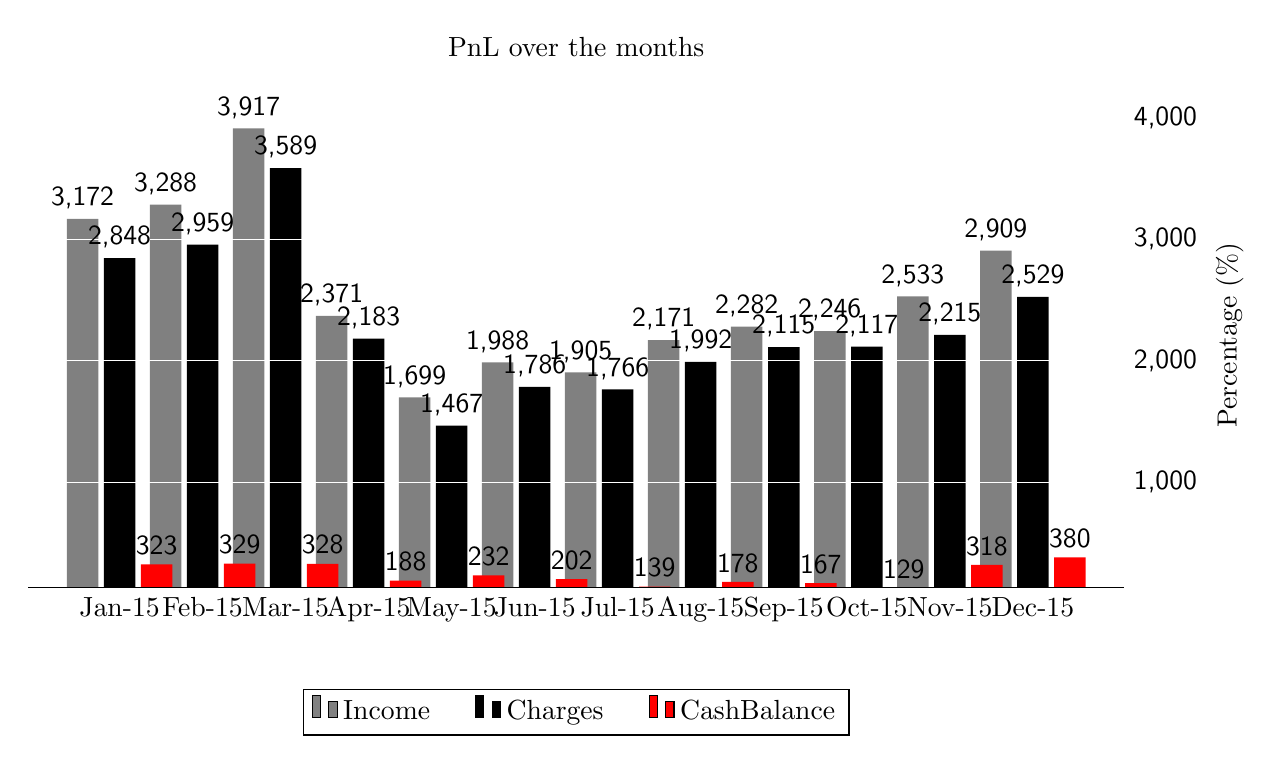
\begin{tikzpicture}[thick, scale=1]
\begin{axis}[
title={Kapital over time},
ybar, axis on top,
title={PnL over the months},
height=8cm, width=15.5cm,
bar width=0.4cm,
ymajorgrids, tick align=inside,
major grid style={draw=white},
enlarge y limits={value=.1,upper},
axis x line*=bottom,
axis y line*=right,
y axis line style={opacity=0},
tickwidth=0pt,
enlarge x limits=true,
legend style={
at={(0.5,-0.2)},
anchor=north,
legend columns=-1,
/tikz/every even column/.append style={column sep=0.5cm}
},
ylabel={Percentage (\%)},
symbolic x coords={
xlabel={Time [Days]},
ylabel={Kapital [euro]},
ymin=-4.956,ymax=27.836,
Jan-15,Feb-15,Mar-15,Apr-15,May-15,Jun-15,Jul-15,Aug-15,Sep-15,Oct-15,Nov-15,Dec-15},xtick=data,
nodes near coords={
\pgfmathprintnumber[precision=0]{\pgfplotspointmeta}
}
]
\addplot [draw=none, fill=black!50] coordinates {
(Jan-15,3171.67)
(Feb-15,3288.125)
(Mar-15,3916.859)
(Apr-15,2371.335)
(May-15,1699.039)
(Jun-15,1987.688)
(Jul-15,1904.966)
(Aug-15,2170.602)
(Sep-15,2281.823)
(Oct-15,2246.281)
(Nov-15,2533.229)
(Dec-15,2908.756)
};
\addplot [draw=none, fill=black!100] coordinates {
(Jan-15,2848.301)
(Feb-15,2958.914)
(Mar-15,3589.333)
(Apr-15,2183.188)
(May-15,1467.326)
(Jun-15,1785.85)
(Jul-15,1766.312)
(Aug-15,1992.222)
(Sep-15,2114.79)
(Oct-15,2117.486)
(Nov-15,2215.477)
(Dec-15,2528.859)
};
\addplot [draw=none, fill=red!100] coordinates {
(Jan-15,323.369)
(Feb-15,329.211)
(Mar-15,327.526)
(Apr-15,188.147)
(May-15,231.713)
(Jun-15,201.838)
(Jul-15,138.654)
(Aug-15,178.38)
(Sep-15,167.033)
(Oct-15,128.795)
(Nov-15,317.752)
(Dec-15,379.897)
};

\legend{Income,Charges,CashBalance}
\end{axis}
\end{tikzpicture}


We need for each graph a table referencing the perl script, the period and the table used for the data.\\
Below is the beginning of the code generating this graph
\lstinputlisting[language=Octave, firstline=3, lastline=5]{../Perl/readCharges}

%{\footnotesize
%BarPlotPnl
%}
\subsubsection{PnL}
%\input{BarPlotPnL}
%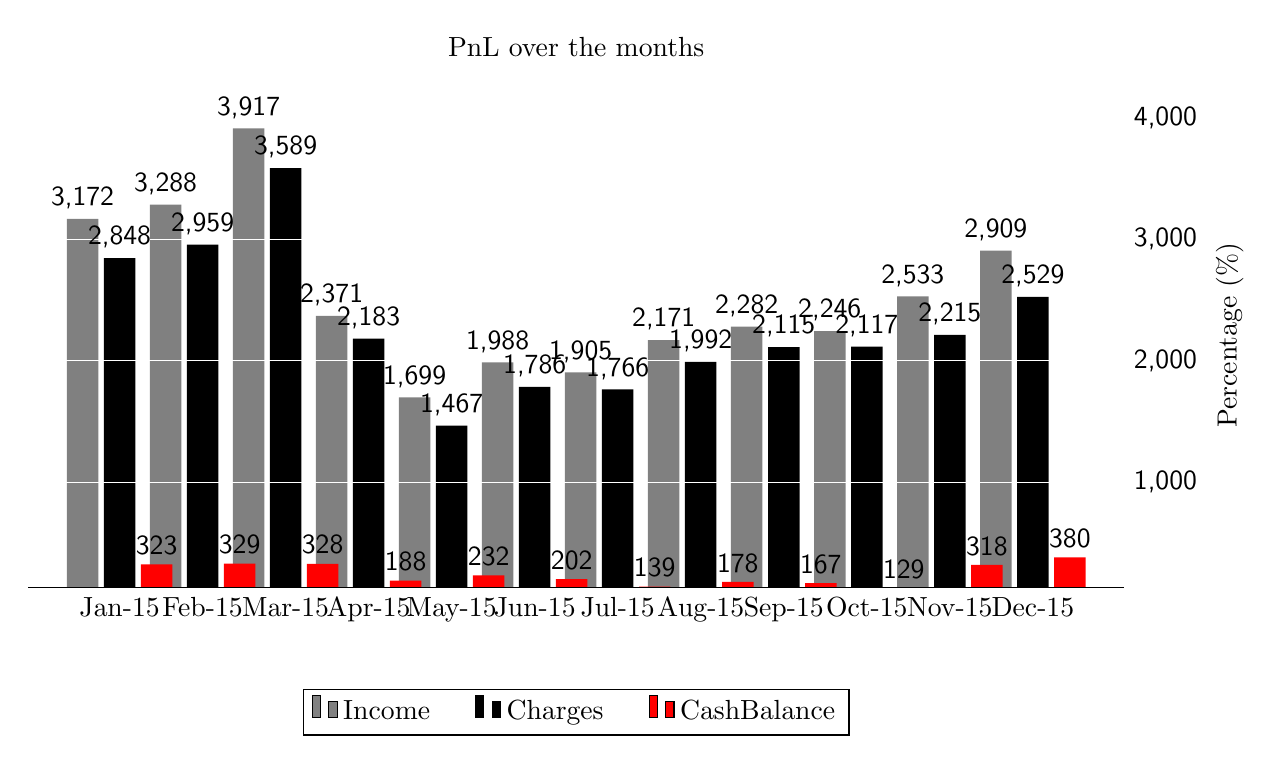
\begin{tikzpicture}[thick, scale=1]
\begin{axis}[
title={Kapital over time},
ybar, axis on top,
title={PnL over the months},
height=8cm, width=15.5cm,
bar width=0.4cm,
ymajorgrids, tick align=inside,
major grid style={draw=white},
enlarge y limits={value=.1,upper},
axis x line*=bottom,
axis y line*=right,
y axis line style={opacity=0},
tickwidth=0pt,
enlarge x limits=true,
legend style={
at={(0.5,-0.2)},
anchor=north,
legend columns=-1,
/tikz/every even column/.append style={column sep=0.5cm}
},
ylabel={Percentage (\%)},
symbolic x coords={
xlabel={Time [Days]},
ylabel={Kapital [euro]},
ymin=-4.956,ymax=27.836,
Jan-15,Feb-15,Mar-15,Apr-15,May-15,Jun-15,Jul-15,Aug-15,Sep-15,Oct-15,Nov-15,Dec-15},xtick=data,
nodes near coords={
\pgfmathprintnumber[precision=0]{\pgfplotspointmeta}
}
]
\addplot [draw=none, fill=black!50] coordinates {
(Jan-15,3171.67)
(Feb-15,3288.125)
(Mar-15,3916.859)
(Apr-15,2371.335)
(May-15,1699.039)
(Jun-15,1987.688)
(Jul-15,1904.966)
(Aug-15,2170.602)
(Sep-15,2281.823)
(Oct-15,2246.281)
(Nov-15,2533.229)
(Dec-15,2908.756)
};
\addplot [draw=none, fill=black!100] coordinates {
(Jan-15,2848.301)
(Feb-15,2958.914)
(Mar-15,3589.333)
(Apr-15,2183.188)
(May-15,1467.326)
(Jun-15,1785.85)
(Jul-15,1766.312)
(Aug-15,1992.222)
(Sep-15,2114.79)
(Oct-15,2117.486)
(Nov-15,2215.477)
(Dec-15,2528.859)
};
\addplot [draw=none, fill=red!100] coordinates {
(Jan-15,323.369)
(Feb-15,329.211)
(Mar-15,327.526)
(Apr-15,188.147)
(May-15,231.713)
(Jun-15,201.838)
(Jul-15,138.654)
(Aug-15,178.38)
(Sep-15,167.033)
(Oct-15,128.795)
(Nov-15,317.752)
(Dec-15,379.897)
};

\legend{Income,Charges,CashBalance}
\end{axis}
\end{tikzpicture}

What is the point in having the same graph twice on the same page?!\\
\lstinputlisting[language=Octave, firstline=3, lastline=5]{../Perl/readCharges}

\subsubsection{Kapital}

%\input{BarPlotPnL}
FK - Here we have a pb that needs to be sorted 
%\begin{tikzpicture}[thick, scale=1]
\begin{axis}[
title={Kapital over time},
ybar, axis on top,
title={PnL over the months},
height=8cm, width=15.5cm,
bar width=0.4cm,
ymajorgrids, tick align=inside,
major grid style={draw=white},
enlarge y limits={value=.1,upper},
axis x line*=bottom,
axis y line*=right,
y axis line style={opacity=0},
tickwidth=0pt,
enlarge x limits=true,
legend style={
at={(0.5,-0.2)},
anchor=north,
legend columns=-1,
/tikz/every even column/.append style={column sep=0.5cm}
},
ylabel={Percentage (\%)},
symbolic x coords={
xlabel={Time [Days]},
ylabel={Kapital [euro]},
ymin=-11.02157,ymax=21.77043,
Jan-18,Feb-18,Mar-18,Apr-18,May-18,Jun-18,Jul-18,Aug-18,Sep-18,Oct-18,Nov-18,xtick=data,
nodes near coords={
\pgfmathprintnumber[precision=0]{\pgfplotspointmeta}
}
]
\addplot [draw=none, fill=red!100] coordinates {
(Jan-18,-83.8994)
(Feb-18,-46.97312)
(Mar-18,-52.03197)
(Apr-18,-52.81598)
(May-18,-96.81726)
(Jun-18,-87.10997)
(Jul-18,-88.51826)
(Aug-18,-113.91554)
(Sep-18,-107.10126)
(Oct-18,-141.31811)
(Nov-18,-50.46756)
};
\addplot [draw=none, fill=black!100] coordinates {
(Jan-18,468.16)
(Feb-18,374.528)
(Mar-18,491.568)
(Apr-18,327.712)
(May-18,421.344)
(Jun-18,491.568)
(Jul-18,421.344)
(Aug-18,514.976)
(Sep-18,421.344)
(Oct-18,538.384)
(Nov-18,187.264)
};
\addplot [draw=none, fill=black!50] coordinates {
(Jan-18,654.9914)
(Feb-18,523.99312)
(Mar-18,687.74097)
(Apr-18,458.49398)
(May-18,589.49226)
(Jun-18,687.74097)
(Jul-18,589.49226)
(Aug-18,720.49054)
(Sep-18,589.49226)
(Oct-18,753.24011)
(Nov-18,261.99656)
};

\legend{Assets,Liabilities,Kapital}
\end{axis}
\end{tikzpicture}

\subsubsection{Plot of an example}
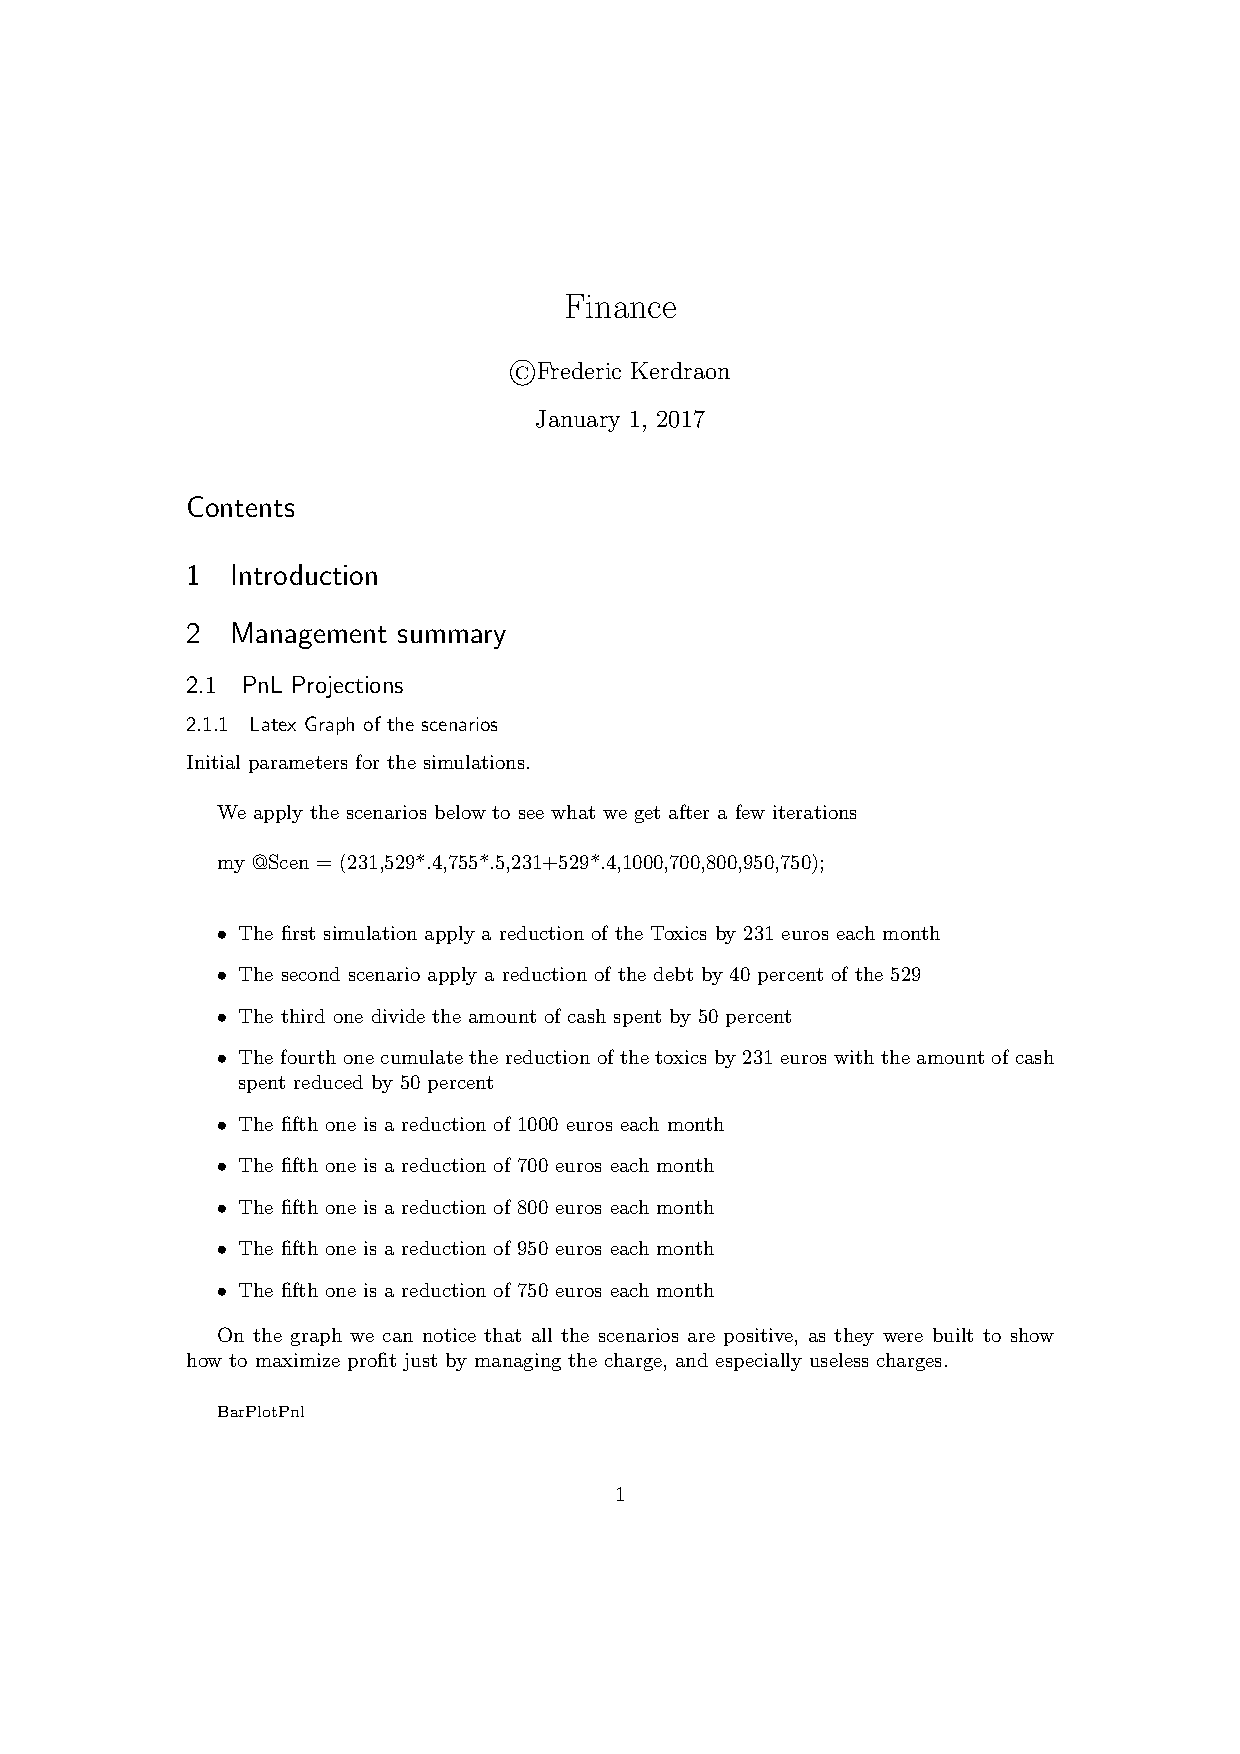
\includegraphics[scale=0.3]{Finance.png}}
How is this graph generated? 
\lstinputlisting[language=Octave, firstline=3, lastline=5]{../Perl/readCharges}
%tableae.dat\\
%file.dat\\
%immigration.dat\\
%finance.dat\\
%charges.dat\\
%article_contourtmp0.dat\\
%Surface4_contourtmp0.dat\\
%pgfplots_scatterdata4.dat\\
%assets.dat\\
%chargesKiviat.dat\\
%resourcesKiviat.dat\\

%\subsubsection{Latex example}
%\input{parabola-plot}

%\subsubsection{Latex example}
%\input{tikzdevice-demo}

%\subsubsection{Latex example}
%\input{TimeTable}

%\subsubsection{Latex example}
%\input{Torn Paper}

%\subsubsection{Latex example}
%\input{Weather Table}

%\subsubsection{Latex example}
%\input{Transparent}

\subsubsection{Cashflows over a limit}
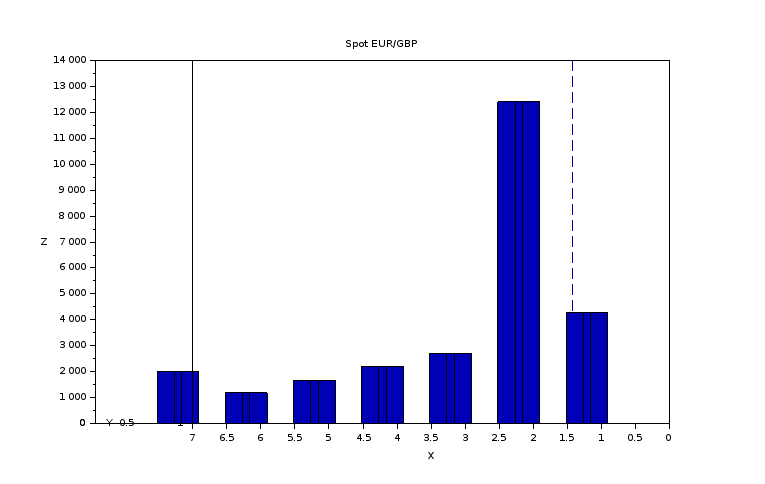
\includegraphics[scale=0.6]{../Maths/Vector.png}
\lstinputlisting[language=Octave, firstline=3, lastline=5]{../Perl/readCharges}

The limit is defined by the variable \$MAXCASHFLOW\\
The latest improvements on the scilab knowledge should be useable here to manage the dates properly.\\

%This where science enter the game as here can call scilab and there is no limit at what we could calculate... fascinating!\\
%How do we populate Scilab with Negative numbers where there are Debits and Positive numbers for the Credit
\subsubsection{Cash balance}
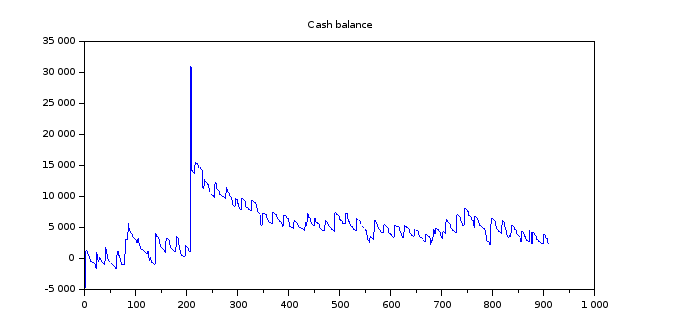
\includegraphics[scale=0.6]{Scilab-cashBalance.png}
\lstinputlisting[language=Octave, firstline=3, lastline=5]{../Perl/readCharges}
The moving average is funny and needs to be corrected.\\
%\includepdf[pages={1}]{stockchart.pdf}
%\includepdf[pages={1}]{friedberg.pdf}
%\subsubsection{Surface}
%\input{PnLSurface}

%\subsubsection{Gaussian Curve}

%\includepdf[pages={1}]{GaussianCurve.pdf}
%\input{GaussianCurve}
%Was removed because very uncomplete...

%\subsubsection{Parabola}
%This I beleive should be the logo for the finance document, so that every doc has it's logo now :-)\\
%\includepdf[pages={1}]{parabola-plotpdf}
%\input{parabola-plot}

%\subsubsection{Weather}
%\includepdf[pages={1}]{WeatherTable.pdf}
%\input{WeatherTable2}

%\subsubsection{Map Of The Charges}
%\includepdf[pages={1}]{MapOfTheCharges.pdf}
%\input{MapOfTheCharges}

\subsubsection{Pnl over time}
The scenarios given in the table are only examples, the real scenarios are provided in the graph below
\begin{longtable}{|c|c|c|c|c|c|}
\hline
\multicolumn{6}{|c|}{Scenarios} \\
\hline
PnL; CumPnL; Tox; Debt(40%); Cash(50%); Tox-Debt(40%)
PnL & CumPnL & Tox & Debt(40\%) & Cash(50\%) & Tox-Debt(40\%)
\hline
472;472;703;684;850;915
472 & 472 & 703 & 684 & 850 & 915\\
\hline
-475;-2;459;420;752;882
-475 & -2 & 459 & 420 & 752 & 882\\
\hline
\end{longtable}

\lstinputlisting[language=Octave, firstline=3, lastline=5]{../Perl/readCharges}

All the figures need to be checked carefully by someone who knows what it's doing.\\
We print only the last 10 PnL meaesures (Need to add a variable for that limit)\\
The first column can be reduced to the PnL as the other ficures appear in the table. Also a limit for this table size should be defined as there could be thousands of scenarios.\\

\subsection{History and extrapolations}

\subsubsection{Kapital curve}
%Kapital trend,Assets trend,Liabilities trend,Leverage trend\\
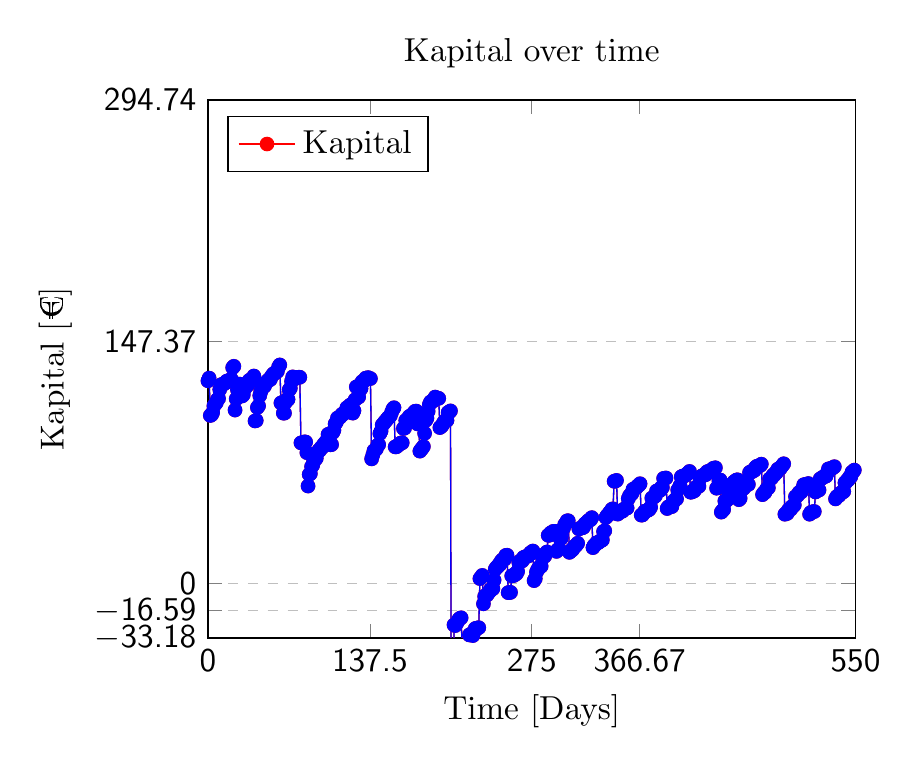
\begin{tikzpicture}[thick, scale=1.2]
\begin{axis}[
title={Kapital over time},
xlabel={Time [Days]},
ylabel={Kapital [\texteuro]},
xmin=0,xmax=550,
ymin=-33.18,ymax=294.74,
xtick={0,137.5,275,366.666666666667,550},
ytick={-33.18,-16.59,0,147.37,294.74},
legend pos=north west,
ymajorgrids=true,
grid style=dashed,
]
\addplot[
color=red,
mark=*,
]
coordinates {
(0,123.51)(1,125.16)(2,102.38)(3,102.78)(4,104.15)(5,108.16)(6,109.35)(7,110.02)(8,112.07)(9,112.68)(10,118.21)(11,121.07)(12,121.25)(13,121.5)(14,121.85)(15,122.55)(16,123.33)(17,123.53)(18,123.67)(19,124.1)(20,124.3)(21,131.53)(22,132.37)(23,105.7)(24,112.5)(25,118.19)(26,119.77)(27,121.53)(28,115.31)(29,114.26)(30,115)(31,118.39)(32,120.38)(33,120.38)(34,121.18)(35,123.73)(36,123.97)(37,124.57)(38,124.66)(39,126.43)(40,99.04)(41,99.31)(42,107.22)(43,108.23)(44,114.51)(45,117.09)(46,119.63)(47,119.99)(48,120.22)(49,122.33)(50,122.77)(51,123.77)(52,124.32)(53,124.32)(54,126.26)(55,127.22)(56,128.02)(57,128.27)(58,128.77)(59,129.37)(60,131.91)(61,133.18)(62,110)(63,110.33)(64,103.83)(65,103.83)(66,110.53)(67,112.14)(68,112.18)(69,118.03)(70,119.01)(71,123.24)(72,125.92)(73,125.46)(74,124.82)(75,125.4)(76,125.63)(77,125.69)(78,125.69)(79,85.69)(80,85.59)(81,86.13)(82,86.27)(83,86.22)(84,79.72)(85,59.38)(86,66.42)(87,66.91)(88,71.22)(89,72.1)(90,74.49)(91,75.69)(92,76.29)(93,79.54)(94,80.98)(95,81.18)(96,82.68)(97,82.88)(98,84.46)(99,85.26)(100,86.27)(101,86.91)(102,90.86)(103,91.01)(104,84.51)(105,84.67)(106,91.95)(107,93.41)(108,97.28)(109,98.23)(110,100.81)(111,100.97)(112,101.25)(113,102.21)(114,103.21)(115,103.21)(116,104.01)(117,105.05)(118,107.12)(119,107.24)(120,107.99)(121,108.85)(122,109.03)(123,103.82)(124,105.33)(125,112.03)(126,119.78)(127,120.06)(128,113.64)(129,118.07)(130,118.75)(131,123.08)(132,123.18)(133,123.78)(134,125.14)(135,124.68)(136,125.5)(137,124.92)(138,124.92)(139,75.92)(140,78.26)(141,80.91)(142,81.37)(143,81.98)(144,84.02)(145,84.63)(146,91.36)(147,92.8)(148,96.63)(149,97.25)(150,98.36)(151,99.12)(152,100.02)(153,100.92)(154,101.54)(155,102.34)(156,104.35)(157,106.24)(158,107.11)(159,83.26)(160,83.27)(161,83.92)(162,84.43)(163,85.23)(164,85.65)(165,85.74)(166,94.51)(167,94.67)(168,99.35)(169,99.65)(170,100.45)(171,101.77)(172,102.08)(173,102.13)(174,103.19)(175,104.12)(176,104.96)(177,105.04)(178,97.26)(179,97.36)(180,80.64)(181,81.64)(182,82.4)(183,83.46)(184,91.52)(185,99.41)(186,100.76)(187,104.91)(188,109)(189,110.58)(190,110.91)(191,111.09)(192,112.3)(193,113.61)(194,112.7)(195,112.85)(196,112.85)(197,95.01)(198,95.61)(199,96.38)(200,97.9)(201,98.91)(202,99.03)(203,99.39)(204,104.27)(205,104.45)(206,105.18)(207,-194.74)(208,-192.18)(209,-25.26)(210,-25.69)(211,-24.59)(212,-23.28)(213,-21.99)(214,-21.26)(215,-20.92)(216,-39.55)(217,-37.95)(218,-37.77)(219,-37.07)(220,-36.96)(221,-36.91)(222,-31.39)(223,-30.94)(224,-30.77)(225,-31.76)(226,-29.56)(227,-27.52)(228,-27.32)(229,-27.15)(230,-26.96)(231,2.95)(232,3.73)(233,4.90000000000001)(234,-12.4)(235,-7.90000000000001)(236,-7.23999999999999)(237,-7.04000000000001)(238,-5.88)(239,-5.09)(240,-3.69)(241,-3.64)(242,-3.16)(243,2.05)(244,8.68000000000001)(245,9.73)(246,10.15)(247,11.45)(248,11.58)(249,13.53)(250,14.37)(251,14.75)(252,14.82)(253,17.09)(254,17.21)(255,-5.61)(256,-5.5)(257,-5.42)(258,4.64)(259,4.79000000000001)(260,4.94)(261,5.86)(262,5.93000000000001)(263,7.36)(264,12.77)(265,13.61)(266,13.68)(267,13.79)(268,15.8)(269,16.09)(270,16.4)(271,16.48)(272,16.74)(273,17.63)(274,18.75)(275,18.86)(276,19.77)(277,1.73)(278,2.92)(279,6.84)(280,8.48999999999999)(281,9.23999999999999)(282,10.3)(283,10.46)(284,15.62)(285,16.34)(286,16.57)(287,18.42)(288,19.22)(289,29.33)(290,29.4)(291,30.74)(292,30.79)(293,31.66)(294,31.71)(295,31.75)(296,19.53)(297,20.48)(298,20.86)(299,27.39)(300,27.45)(301,32.76)(302,33.76)(303,35.89)(304,36.59)(305,38.14)(306,38.22)(307,18.95)(308,20.05)(309,20.15)(310,20.95)(311,22.36)(312,22.74)(313,23.47)(314,24.52)(315,33.29)(316,33.57)(317,33.83)(318,33.92)(319,34.28)(320,36.18)(321,36.73)(322,37.21)(323,38.21)(324,38.63)(325,38.87)(326,40.13)(327,21.83)(328,23.16)(329,23.62)(330,24.76)(331,24.8)(332,25.1)(333,25.74)(334,26.26)(335,26.5)(336,31.66)(337,32.09)(338,40.19)(339,41.32)(340,41.59)(341,43.22)(342,43.51)(343,45.12)(344,45.52)(345,62.28)(346,62.38)(347,62.82)(348,42.27)(349,43.53)(350,43.65)(351,43.9)(352,44.02)(353,45.08)(354,45.56)(355,45.88)(356,45.96)(357,51.7)(358,53.4)(359,54.15)(360,54.74)(361,57.39)(362,57.47)(363,58.07)(364,58.62)(365,59.44)(366,59.9)(367,60.78)(368,41.66)(369,41.74)(370,42.86)(371,44.01)(372,44.07)(373,44.51)(374,44.7)(375,45.3)(376,46.51)(377,52)(378,52.24)(379,53)(380,53.31)(381,56.35)(382,56.56)(383,56.64)(384,56.72)(385,58.41)(386,58.48)(387,64.01)(388,64.12)(389,64.28)(390,45.67)(391,46.65)(392,46.72)(393,46.79)(394,46.87)(395,49.86)(396,50.39)(397,51.29)(398,51.55)(399,56.95)(400,57.95)(401,59.68)(402,64.99)(403,65.41)(404,65.5)(405,65.62)(406,66.29)(407,66.55)(408,67.45)(409,68.27)(410,55.58)(411,55.81)(412,56.13)(413,56.43)(414,58.19)(415,58.93)(416,59.16)(417,59.23)(418,64.36)(419,65.36)(420,65.47)(421,66.14)(422,66.22)(423,66.36)(424,68.12)(425,68.33)(426,68.43)(427,68.56)(428,68.8)(429,70.11)(430,70.28)(431,70.51)(432,58.04)(433,58.44)(434,62.5)(435,63.09)(436,43.48)(437,44.38)(438,45.03)(439,50.22)(440,50.29)(441,50.97)(442,52.68)(443,56.9)(444,57.15)(445,60.54)(446,61.16)(447,62.05)(448,62.4)(449,63.08)(450,63.15)(451,51.06)(452,51.85)(453,57.34)(454,57.59)(455,57.98)(456,59.1)(457,60.18)(458,60.31)(459,60.38)(460,67.63)(461,68)(462,68.07)(463,68.84)(464,68.87)(465,70.63)(466,71.34)(467,71.56)(468,71.64)(469,71.87)(470,72.7)(471,54.12)(472,55.2)(473,55.38)(474,56.94)(475,58.14)(476,58.3)(477,63.68)(478,63.83)(479,64.52)(480,66.08)(481,66.15)(482,67.41)(483,67.71)(484,69.64)(485,69.88)(486,70.03)(487,71.1)(488,71.99)(489,72.96)(490,42.18)(491,42.78)(492,42.67)(493,44.76)(494,44.91)(495,45.24)(496,46.86)(497,47.11)(498,47.8)(499,52.89)(500,53.18)(501,53.86)(502,55.38)(503,55.64)(504,55.86)(505,57.68)(506,60.15)(507,60.23)(508,60.34)(509,60.63)(510,60.9)(511,42.21)(512,43.26)(513,43.48)(514,43.73)(515,43.86)(516,55.74)(517,56.8)(518,56.84)(519,56.95)(520,63.77)(521,63.85)(522,64.7)(523,64.94)(524,65.23)(525,65.45)(526,67.38)(527,69.83)(528,69.9)(529,69.99)(530,70.08)(531,70.73)(532,71.18)(533,51.53)(534,52.84)(535,53.33)(536,53.6)(537,54.97)(538,55.33)(539,55.6)(540,56.07)(541,61.36)(542,61.82)(543,63.04)(544,63.24)(545,64.94)(546,65.01)(547,67.83)(548,68.15)(549,69.1)
};
\addplot[
color=blue,
mark=*,
]
coordinates {
(0,123.51)(1,125.16)(2,102.38)(3,102.78)(4,104.15)(5,108.16)(6,109.35)(7,110.02)(8,112.07)(9,112.68)(10,118.21)(11,121.07)(12,121.25)(13,121.5)(14,121.85)(15,122.55)(16,123.33)(17,123.53)(18,123.67)(19,124.1)(20,124.3)(21,131.53)(22,132.37)(23,105.7)(24,112.5)(25,118.19)(26,119.77)(27,121.53)(28,115.31)(29,114.26)(30,115)(31,118.39)(32,120.38)(33,120.38)(34,121.18)(35,123.73)(36,123.97)(37,124.57)(38,124.66)(39,126.43)(40,99.04)(41,99.31)(42,107.22)(43,108.23)(44,114.51)(45,117.09)(46,119.63)(47,119.99)(48,120.22)(49,122.33)(50,122.77)(51,123.77)(52,124.32)(53,124.32)(54,126.26)(55,127.22)(56,128.02)(57,128.27)(58,128.77)(59,129.37)(60,131.91)(61,133.18)(62,110)(63,110.33)(64,103.83)(65,103.83)(66,110.53)(67,112.14)(68,112.18)(69,118.03)(70,119.01)(71,123.24)(72,125.92)(73,125.46)(74,124.82)(75,125.4)(76,125.63)(77,125.69)(78,125.69)(79,85.69)(80,85.59)(81,86.13)(82,86.27)(83,86.22)(84,79.72)(85,59.38)(86,66.42)(87,66.91)(88,71.22)(89,72.1)(90,74.49)(91,75.69)(92,76.29)(93,79.54)(94,80.98)(95,81.18)(96,82.68)(97,82.88)(98,84.46)(99,85.26)(100,86.27)(101,86.91)(102,90.86)(103,91.01)(104,84.51)(105,84.67)(106,91.95)(107,93.41)(108,97.28)(109,98.23)(110,100.81)(111,100.97)(112,101.25)(113,102.21)(114,103.21)(115,103.21)(116,104.01)(117,105.05)(118,107.12)(119,107.24)(120,107.99)(121,108.85)(122,109.03)(123,103.82)(124,105.33)(125,112.03)(126,119.78)(127,120.06)(128,113.64)(129,118.07)(130,118.75)(131,123.08)(132,123.18)(133,123.78)(134,125.14)(135,124.68)(136,125.5)(137,124.92)(138,124.92)(139,75.92)(140,78.26)(141,80.91)(142,81.37)(143,81.98)(144,84.02)(145,84.63)(146,91.36)(147,92.8)(148,96.63)(149,97.25)(150,98.36)(151,99.12)(152,100.02)(153,100.92)(154,101.54)(155,102.34)(156,104.35)(157,106.24)(158,107.11)(159,83.26)(160,83.27)(161,83.92)(162,84.43)(163,85.23)(164,85.65)(165,85.74)(166,94.51)(167,94.67)(168,99.35)(169,99.65)(170,100.45)(171,101.77)(172,102.08)(173,102.13)(174,103.19)(175,104.12)(176,104.96)(177,105.04)(178,97.26)(179,97.36)(180,80.64)(181,81.64)(182,82.4)(183,83.46)(184,91.52)(185,99.41)(186,100.76)(187,104.91)(188,109)(189,110.58)(190,110.91)(191,111.09)(192,112.3)(193,113.61)(194,112.7)(195,112.85)(196,112.85)(197,95.01)(198,95.61)(199,96.38)(200,97.9)(201,98.91)(202,99.03)(203,99.39)(204,104.27)(205,104.45)(206,105.18)(207,-194.74)(208,-192.18)(209,-25.26)(210,-25.69)(211,-24.59)(212,-23.28)(213,-21.99)(214,-21.26)(215,-20.92)(216,-39.55)(217,-37.95)(218,-37.77)(219,-37.07)(220,-36.96)(221,-36.91)(222,-31.39)(223,-30.94)(224,-30.77)(225,-31.76)(226,-29.56)(227,-27.52)(228,-27.32)(229,-27.15)(230,-26.96)(231,2.95)(232,3.73)(233,4.90000000000001)(234,-12.4)(235,-7.90000000000001)(236,-7.23999999999999)(237,-7.04000000000001)(238,-5.88)(239,-5.09)(240,-3.69)(241,-3.64)(242,-3.16)(243,2.05)(244,8.68000000000001)(245,9.73)(246,10.15)(247,11.45)(248,11.58)(249,13.53)(250,14.37)(251,14.75)(252,14.82)(253,17.09)(254,17.21)(255,-5.61)(256,-5.5)(257,-5.42)(258,4.64)(259,4.79000000000001)(260,4.94)(261,5.86)(262,5.93000000000001)(263,7.36)(264,12.77)(265,13.61)(266,13.68)(267,13.79)(268,15.8)(269,16.09)(270,16.4)(271,16.48)(272,16.74)(273,17.63)(274,18.75)(275,18.86)(276,19.77)(277,1.73)(278,2.92)(279,6.84)(280,8.48999999999999)(281,9.23999999999999)(282,10.3)(283,10.46)(284,15.62)(285,16.34)(286,16.57)(287,18.42)(288,19.22)(289,29.33)(290,29.4)(291,30.74)(292,30.79)(293,31.66)(294,31.71)(295,31.75)(296,19.53)(297,20.48)(298,20.86)(299,27.39)(300,27.45)(301,32.76)(302,33.76)(303,35.89)(304,36.59)(305,38.14)(306,38.22)(307,18.95)(308,20.05)(309,20.15)(310,20.95)(311,22.36)(312,22.74)(313,23.47)(314,24.52)(315,33.29)(316,33.57)(317,33.83)(318,33.92)(319,34.28)(320,36.18)(321,36.73)(322,37.21)(323,38.21)(324,38.63)(325,38.87)(326,40.13)(327,21.83)(328,23.16)(329,23.62)(330,24.76)(331,24.8)(332,25.1)(333,25.74)(334,26.26)(335,26.5)(336,31.66)(337,32.09)(338,40.19)(339,41.32)(340,41.59)(341,43.22)(342,43.51)(343,45.12)(344,45.52)(345,62.28)(346,62.38)(347,62.82)(348,42.27)(349,43.53)(350,43.65)(351,43.9)(352,44.02)(353,45.08)(354,45.56)(355,45.88)(356,45.96)(357,51.7)(358,53.4)(359,54.15)(360,54.74)(361,57.39)(362,57.47)(363,58.07)(364,58.62)(365,59.44)(366,59.9)(367,60.78)(368,41.66)(369,41.74)(370,42.86)(371,44.01)(372,44.07)(373,44.51)(374,44.7)(375,45.3)(376,46.51)(377,52)(378,52.24)(379,53)(380,53.31)(381,56.35)(382,56.56)(383,56.64)(384,56.72)(385,58.41)(386,58.48)(387,64.01)(388,64.12)(389,64.28)(390,45.67)(391,46.65)(392,46.72)(393,46.79)(394,46.87)(395,49.86)(396,50.39)(397,51.29)(398,51.55)(399,56.95)(400,57.95)(401,59.68)(402,64.99)(403,65.41)(404,65.5)(405,65.62)(406,66.29)(407,66.55)(408,67.45)(409,68.27)(410,55.58)(411,55.81)(412,56.13)(413,56.43)(414,58.19)(415,58.93)(416,59.16)(417,59.23)(418,64.36)(419,65.36)(420,65.47)(421,66.14)(422,66.22)(423,66.36)(424,68.12)(425,68.33)(426,68.43)(427,68.56)(428,68.8)(429,70.11)(430,70.28)(431,70.51)(432,58.04)(433,58.44)(434,62.5)(435,63.09)(436,43.48)(437,44.38)(438,45.03)(439,50.22)(440,50.29)(441,50.97)(442,52.68)(443,56.9)(444,57.15)(445,60.54)(446,61.16)(447,62.05)(448,62.4)(449,63.08)(450,63.15)(451,51.06)(452,51.85)(453,57.34)(454,57.59)(455,57.98)(456,59.1)(457,60.18)(458,60.31)(459,60.38)(460,67.63)(461,68)(462,68.07)(463,68.84)(464,68.87)(465,70.63)(466,71.34)(467,71.56)(468,71.64)(469,71.87)(470,72.7)(471,54.12)(472,55.2)(473,55.38)(474,56.94)(475,58.14)(476,58.3)(477,63.68)(478,63.83)(479,64.52)(480,66.08)(481,66.15)(482,67.41)(483,67.71)(484,69.64)(485,69.88)(486,70.03)(487,71.1)(488,71.99)(489,72.96)(490,42.18)(491,42.78)(492,42.67)(493,44.76)(494,44.91)(495,45.24)(496,46.86)(497,47.11)(498,47.8)(499,52.89)(500,53.18)(501,53.86)(502,55.38)(503,55.64)(504,55.86)(505,57.68)(506,60.15)(507,60.23)(508,60.34)(509,60.63)(510,60.9)(511,42.21)(512,43.26)(513,43.48)(514,43.73)(515,43.86)(516,55.74)(517,56.8)(518,56.84)(519,56.95)(520,63.77)(521,63.85)(522,64.7)(523,64.94)(524,65.23)(525,65.45)(526,67.38)(527,69.83)(528,69.9)(529,69.99)(530,70.08)(531,70.73)(532,71.18)(533,51.53)(534,52.84)(535,53.33)(536,53.6)(537,54.97)(538,55.33)(539,55.6)(540,56.07)(541,61.36)(542,61.82)(543,63.04)(544,63.24)(545,64.94)(546,65.01)(547,67.83)(548,68.15)(549,69.1)
};
\legend{Kapital}
\end{axis}
\end{tikzpicture}

\lstinputlisting[language=Octave, firstline=3, lastline=5]{../Perl/readCharges}

This is the kapitalCurve from perl\\ Doesn't work at the moment...\\

\subsubsection{PnL curve}
\input{pnlCurve}
\lstinputlisting[language=Octave, firstline=3, lastline=5]{../Perl/readCharges}
This is the pnlCurve from perl. Doesn't seem to be working?! What is it supposed to show?\\
%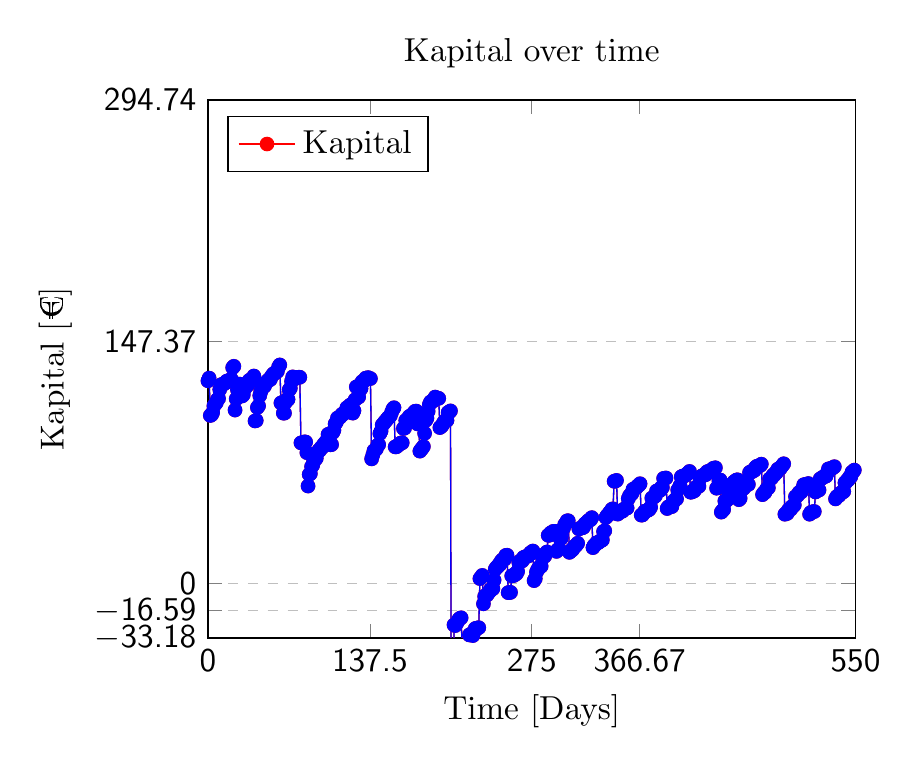
\begin{tikzpicture}[thick, scale=1.2]
\begin{axis}[
title={Kapital over time},
xlabel={Time [Days]},
ylabel={Kapital [\texteuro]},
xmin=0,xmax=550,
ymin=-33.18,ymax=294.74,
xtick={0,137.5,275,366.666666666667,550},
ytick={-33.18,-16.59,0,147.37,294.74},
legend pos=north west,
ymajorgrids=true,
grid style=dashed,
]
\addplot[
color=red,
mark=*,
]
coordinates {
(0,123.51)(1,125.16)(2,102.38)(3,102.78)(4,104.15)(5,108.16)(6,109.35)(7,110.02)(8,112.07)(9,112.68)(10,118.21)(11,121.07)(12,121.25)(13,121.5)(14,121.85)(15,122.55)(16,123.33)(17,123.53)(18,123.67)(19,124.1)(20,124.3)(21,131.53)(22,132.37)(23,105.7)(24,112.5)(25,118.19)(26,119.77)(27,121.53)(28,115.31)(29,114.26)(30,115)(31,118.39)(32,120.38)(33,120.38)(34,121.18)(35,123.73)(36,123.97)(37,124.57)(38,124.66)(39,126.43)(40,99.04)(41,99.31)(42,107.22)(43,108.23)(44,114.51)(45,117.09)(46,119.63)(47,119.99)(48,120.22)(49,122.33)(50,122.77)(51,123.77)(52,124.32)(53,124.32)(54,126.26)(55,127.22)(56,128.02)(57,128.27)(58,128.77)(59,129.37)(60,131.91)(61,133.18)(62,110)(63,110.33)(64,103.83)(65,103.83)(66,110.53)(67,112.14)(68,112.18)(69,118.03)(70,119.01)(71,123.24)(72,125.92)(73,125.46)(74,124.82)(75,125.4)(76,125.63)(77,125.69)(78,125.69)(79,85.69)(80,85.59)(81,86.13)(82,86.27)(83,86.22)(84,79.72)(85,59.38)(86,66.42)(87,66.91)(88,71.22)(89,72.1)(90,74.49)(91,75.69)(92,76.29)(93,79.54)(94,80.98)(95,81.18)(96,82.68)(97,82.88)(98,84.46)(99,85.26)(100,86.27)(101,86.91)(102,90.86)(103,91.01)(104,84.51)(105,84.67)(106,91.95)(107,93.41)(108,97.28)(109,98.23)(110,100.81)(111,100.97)(112,101.25)(113,102.21)(114,103.21)(115,103.21)(116,104.01)(117,105.05)(118,107.12)(119,107.24)(120,107.99)(121,108.85)(122,109.03)(123,103.82)(124,105.33)(125,112.03)(126,119.78)(127,120.06)(128,113.64)(129,118.07)(130,118.75)(131,123.08)(132,123.18)(133,123.78)(134,125.14)(135,124.68)(136,125.5)(137,124.92)(138,124.92)(139,75.92)(140,78.26)(141,80.91)(142,81.37)(143,81.98)(144,84.02)(145,84.63)(146,91.36)(147,92.8)(148,96.63)(149,97.25)(150,98.36)(151,99.12)(152,100.02)(153,100.92)(154,101.54)(155,102.34)(156,104.35)(157,106.24)(158,107.11)(159,83.26)(160,83.27)(161,83.92)(162,84.43)(163,85.23)(164,85.65)(165,85.74)(166,94.51)(167,94.67)(168,99.35)(169,99.65)(170,100.45)(171,101.77)(172,102.08)(173,102.13)(174,103.19)(175,104.12)(176,104.96)(177,105.04)(178,97.26)(179,97.36)(180,80.64)(181,81.64)(182,82.4)(183,83.46)(184,91.52)(185,99.41)(186,100.76)(187,104.91)(188,109)(189,110.58)(190,110.91)(191,111.09)(192,112.3)(193,113.61)(194,112.7)(195,112.85)(196,112.85)(197,95.01)(198,95.61)(199,96.38)(200,97.9)(201,98.91)(202,99.03)(203,99.39)(204,104.27)(205,104.45)(206,105.18)(207,-194.74)(208,-192.18)(209,-25.26)(210,-25.69)(211,-24.59)(212,-23.28)(213,-21.99)(214,-21.26)(215,-20.92)(216,-39.55)(217,-37.95)(218,-37.77)(219,-37.07)(220,-36.96)(221,-36.91)(222,-31.39)(223,-30.94)(224,-30.77)(225,-31.76)(226,-29.56)(227,-27.52)(228,-27.32)(229,-27.15)(230,-26.96)(231,2.95)(232,3.73)(233,4.90000000000001)(234,-12.4)(235,-7.90000000000001)(236,-7.23999999999999)(237,-7.04000000000001)(238,-5.88)(239,-5.09)(240,-3.69)(241,-3.64)(242,-3.16)(243,2.05)(244,8.68000000000001)(245,9.73)(246,10.15)(247,11.45)(248,11.58)(249,13.53)(250,14.37)(251,14.75)(252,14.82)(253,17.09)(254,17.21)(255,-5.61)(256,-5.5)(257,-5.42)(258,4.64)(259,4.79000000000001)(260,4.94)(261,5.86)(262,5.93000000000001)(263,7.36)(264,12.77)(265,13.61)(266,13.68)(267,13.79)(268,15.8)(269,16.09)(270,16.4)(271,16.48)(272,16.74)(273,17.63)(274,18.75)(275,18.86)(276,19.77)(277,1.73)(278,2.92)(279,6.84)(280,8.48999999999999)(281,9.23999999999999)(282,10.3)(283,10.46)(284,15.62)(285,16.34)(286,16.57)(287,18.42)(288,19.22)(289,29.33)(290,29.4)(291,30.74)(292,30.79)(293,31.66)(294,31.71)(295,31.75)(296,19.53)(297,20.48)(298,20.86)(299,27.39)(300,27.45)(301,32.76)(302,33.76)(303,35.89)(304,36.59)(305,38.14)(306,38.22)(307,18.95)(308,20.05)(309,20.15)(310,20.95)(311,22.36)(312,22.74)(313,23.47)(314,24.52)(315,33.29)(316,33.57)(317,33.83)(318,33.92)(319,34.28)(320,36.18)(321,36.73)(322,37.21)(323,38.21)(324,38.63)(325,38.87)(326,40.13)(327,21.83)(328,23.16)(329,23.62)(330,24.76)(331,24.8)(332,25.1)(333,25.74)(334,26.26)(335,26.5)(336,31.66)(337,32.09)(338,40.19)(339,41.32)(340,41.59)(341,43.22)(342,43.51)(343,45.12)(344,45.52)(345,62.28)(346,62.38)(347,62.82)(348,42.27)(349,43.53)(350,43.65)(351,43.9)(352,44.02)(353,45.08)(354,45.56)(355,45.88)(356,45.96)(357,51.7)(358,53.4)(359,54.15)(360,54.74)(361,57.39)(362,57.47)(363,58.07)(364,58.62)(365,59.44)(366,59.9)(367,60.78)(368,41.66)(369,41.74)(370,42.86)(371,44.01)(372,44.07)(373,44.51)(374,44.7)(375,45.3)(376,46.51)(377,52)(378,52.24)(379,53)(380,53.31)(381,56.35)(382,56.56)(383,56.64)(384,56.72)(385,58.41)(386,58.48)(387,64.01)(388,64.12)(389,64.28)(390,45.67)(391,46.65)(392,46.72)(393,46.79)(394,46.87)(395,49.86)(396,50.39)(397,51.29)(398,51.55)(399,56.95)(400,57.95)(401,59.68)(402,64.99)(403,65.41)(404,65.5)(405,65.62)(406,66.29)(407,66.55)(408,67.45)(409,68.27)(410,55.58)(411,55.81)(412,56.13)(413,56.43)(414,58.19)(415,58.93)(416,59.16)(417,59.23)(418,64.36)(419,65.36)(420,65.47)(421,66.14)(422,66.22)(423,66.36)(424,68.12)(425,68.33)(426,68.43)(427,68.56)(428,68.8)(429,70.11)(430,70.28)(431,70.51)(432,58.04)(433,58.44)(434,62.5)(435,63.09)(436,43.48)(437,44.38)(438,45.03)(439,50.22)(440,50.29)(441,50.97)(442,52.68)(443,56.9)(444,57.15)(445,60.54)(446,61.16)(447,62.05)(448,62.4)(449,63.08)(450,63.15)(451,51.06)(452,51.85)(453,57.34)(454,57.59)(455,57.98)(456,59.1)(457,60.18)(458,60.31)(459,60.38)(460,67.63)(461,68)(462,68.07)(463,68.84)(464,68.87)(465,70.63)(466,71.34)(467,71.56)(468,71.64)(469,71.87)(470,72.7)(471,54.12)(472,55.2)(473,55.38)(474,56.94)(475,58.14)(476,58.3)(477,63.68)(478,63.83)(479,64.52)(480,66.08)(481,66.15)(482,67.41)(483,67.71)(484,69.64)(485,69.88)(486,70.03)(487,71.1)(488,71.99)(489,72.96)(490,42.18)(491,42.78)(492,42.67)(493,44.76)(494,44.91)(495,45.24)(496,46.86)(497,47.11)(498,47.8)(499,52.89)(500,53.18)(501,53.86)(502,55.38)(503,55.64)(504,55.86)(505,57.68)(506,60.15)(507,60.23)(508,60.34)(509,60.63)(510,60.9)(511,42.21)(512,43.26)(513,43.48)(514,43.73)(515,43.86)(516,55.74)(517,56.8)(518,56.84)(519,56.95)(520,63.77)(521,63.85)(522,64.7)(523,64.94)(524,65.23)(525,65.45)(526,67.38)(527,69.83)(528,69.9)(529,69.99)(530,70.08)(531,70.73)(532,71.18)(533,51.53)(534,52.84)(535,53.33)(536,53.6)(537,54.97)(538,55.33)(539,55.6)(540,56.07)(541,61.36)(542,61.82)(543,63.04)(544,63.24)(545,64.94)(546,65.01)(547,67.83)(548,68.15)(549,69.1)
};
\addplot[
color=blue,
mark=*,
]
coordinates {
(0,123.51)(1,125.16)(2,102.38)(3,102.78)(4,104.15)(5,108.16)(6,109.35)(7,110.02)(8,112.07)(9,112.68)(10,118.21)(11,121.07)(12,121.25)(13,121.5)(14,121.85)(15,122.55)(16,123.33)(17,123.53)(18,123.67)(19,124.1)(20,124.3)(21,131.53)(22,132.37)(23,105.7)(24,112.5)(25,118.19)(26,119.77)(27,121.53)(28,115.31)(29,114.26)(30,115)(31,118.39)(32,120.38)(33,120.38)(34,121.18)(35,123.73)(36,123.97)(37,124.57)(38,124.66)(39,126.43)(40,99.04)(41,99.31)(42,107.22)(43,108.23)(44,114.51)(45,117.09)(46,119.63)(47,119.99)(48,120.22)(49,122.33)(50,122.77)(51,123.77)(52,124.32)(53,124.32)(54,126.26)(55,127.22)(56,128.02)(57,128.27)(58,128.77)(59,129.37)(60,131.91)(61,133.18)(62,110)(63,110.33)(64,103.83)(65,103.83)(66,110.53)(67,112.14)(68,112.18)(69,118.03)(70,119.01)(71,123.24)(72,125.92)(73,125.46)(74,124.82)(75,125.4)(76,125.63)(77,125.69)(78,125.69)(79,85.69)(80,85.59)(81,86.13)(82,86.27)(83,86.22)(84,79.72)(85,59.38)(86,66.42)(87,66.91)(88,71.22)(89,72.1)(90,74.49)(91,75.69)(92,76.29)(93,79.54)(94,80.98)(95,81.18)(96,82.68)(97,82.88)(98,84.46)(99,85.26)(100,86.27)(101,86.91)(102,90.86)(103,91.01)(104,84.51)(105,84.67)(106,91.95)(107,93.41)(108,97.28)(109,98.23)(110,100.81)(111,100.97)(112,101.25)(113,102.21)(114,103.21)(115,103.21)(116,104.01)(117,105.05)(118,107.12)(119,107.24)(120,107.99)(121,108.85)(122,109.03)(123,103.82)(124,105.33)(125,112.03)(126,119.78)(127,120.06)(128,113.64)(129,118.07)(130,118.75)(131,123.08)(132,123.18)(133,123.78)(134,125.14)(135,124.68)(136,125.5)(137,124.92)(138,124.92)(139,75.92)(140,78.26)(141,80.91)(142,81.37)(143,81.98)(144,84.02)(145,84.63)(146,91.36)(147,92.8)(148,96.63)(149,97.25)(150,98.36)(151,99.12)(152,100.02)(153,100.92)(154,101.54)(155,102.34)(156,104.35)(157,106.24)(158,107.11)(159,83.26)(160,83.27)(161,83.92)(162,84.43)(163,85.23)(164,85.65)(165,85.74)(166,94.51)(167,94.67)(168,99.35)(169,99.65)(170,100.45)(171,101.77)(172,102.08)(173,102.13)(174,103.19)(175,104.12)(176,104.96)(177,105.04)(178,97.26)(179,97.36)(180,80.64)(181,81.64)(182,82.4)(183,83.46)(184,91.52)(185,99.41)(186,100.76)(187,104.91)(188,109)(189,110.58)(190,110.91)(191,111.09)(192,112.3)(193,113.61)(194,112.7)(195,112.85)(196,112.85)(197,95.01)(198,95.61)(199,96.38)(200,97.9)(201,98.91)(202,99.03)(203,99.39)(204,104.27)(205,104.45)(206,105.18)(207,-194.74)(208,-192.18)(209,-25.26)(210,-25.69)(211,-24.59)(212,-23.28)(213,-21.99)(214,-21.26)(215,-20.92)(216,-39.55)(217,-37.95)(218,-37.77)(219,-37.07)(220,-36.96)(221,-36.91)(222,-31.39)(223,-30.94)(224,-30.77)(225,-31.76)(226,-29.56)(227,-27.52)(228,-27.32)(229,-27.15)(230,-26.96)(231,2.95)(232,3.73)(233,4.90000000000001)(234,-12.4)(235,-7.90000000000001)(236,-7.23999999999999)(237,-7.04000000000001)(238,-5.88)(239,-5.09)(240,-3.69)(241,-3.64)(242,-3.16)(243,2.05)(244,8.68000000000001)(245,9.73)(246,10.15)(247,11.45)(248,11.58)(249,13.53)(250,14.37)(251,14.75)(252,14.82)(253,17.09)(254,17.21)(255,-5.61)(256,-5.5)(257,-5.42)(258,4.64)(259,4.79000000000001)(260,4.94)(261,5.86)(262,5.93000000000001)(263,7.36)(264,12.77)(265,13.61)(266,13.68)(267,13.79)(268,15.8)(269,16.09)(270,16.4)(271,16.48)(272,16.74)(273,17.63)(274,18.75)(275,18.86)(276,19.77)(277,1.73)(278,2.92)(279,6.84)(280,8.48999999999999)(281,9.23999999999999)(282,10.3)(283,10.46)(284,15.62)(285,16.34)(286,16.57)(287,18.42)(288,19.22)(289,29.33)(290,29.4)(291,30.74)(292,30.79)(293,31.66)(294,31.71)(295,31.75)(296,19.53)(297,20.48)(298,20.86)(299,27.39)(300,27.45)(301,32.76)(302,33.76)(303,35.89)(304,36.59)(305,38.14)(306,38.22)(307,18.95)(308,20.05)(309,20.15)(310,20.95)(311,22.36)(312,22.74)(313,23.47)(314,24.52)(315,33.29)(316,33.57)(317,33.83)(318,33.92)(319,34.28)(320,36.18)(321,36.73)(322,37.21)(323,38.21)(324,38.63)(325,38.87)(326,40.13)(327,21.83)(328,23.16)(329,23.62)(330,24.76)(331,24.8)(332,25.1)(333,25.74)(334,26.26)(335,26.5)(336,31.66)(337,32.09)(338,40.19)(339,41.32)(340,41.59)(341,43.22)(342,43.51)(343,45.12)(344,45.52)(345,62.28)(346,62.38)(347,62.82)(348,42.27)(349,43.53)(350,43.65)(351,43.9)(352,44.02)(353,45.08)(354,45.56)(355,45.88)(356,45.96)(357,51.7)(358,53.4)(359,54.15)(360,54.74)(361,57.39)(362,57.47)(363,58.07)(364,58.62)(365,59.44)(366,59.9)(367,60.78)(368,41.66)(369,41.74)(370,42.86)(371,44.01)(372,44.07)(373,44.51)(374,44.7)(375,45.3)(376,46.51)(377,52)(378,52.24)(379,53)(380,53.31)(381,56.35)(382,56.56)(383,56.64)(384,56.72)(385,58.41)(386,58.48)(387,64.01)(388,64.12)(389,64.28)(390,45.67)(391,46.65)(392,46.72)(393,46.79)(394,46.87)(395,49.86)(396,50.39)(397,51.29)(398,51.55)(399,56.95)(400,57.95)(401,59.68)(402,64.99)(403,65.41)(404,65.5)(405,65.62)(406,66.29)(407,66.55)(408,67.45)(409,68.27)(410,55.58)(411,55.81)(412,56.13)(413,56.43)(414,58.19)(415,58.93)(416,59.16)(417,59.23)(418,64.36)(419,65.36)(420,65.47)(421,66.14)(422,66.22)(423,66.36)(424,68.12)(425,68.33)(426,68.43)(427,68.56)(428,68.8)(429,70.11)(430,70.28)(431,70.51)(432,58.04)(433,58.44)(434,62.5)(435,63.09)(436,43.48)(437,44.38)(438,45.03)(439,50.22)(440,50.29)(441,50.97)(442,52.68)(443,56.9)(444,57.15)(445,60.54)(446,61.16)(447,62.05)(448,62.4)(449,63.08)(450,63.15)(451,51.06)(452,51.85)(453,57.34)(454,57.59)(455,57.98)(456,59.1)(457,60.18)(458,60.31)(459,60.38)(460,67.63)(461,68)(462,68.07)(463,68.84)(464,68.87)(465,70.63)(466,71.34)(467,71.56)(468,71.64)(469,71.87)(470,72.7)(471,54.12)(472,55.2)(473,55.38)(474,56.94)(475,58.14)(476,58.3)(477,63.68)(478,63.83)(479,64.52)(480,66.08)(481,66.15)(482,67.41)(483,67.71)(484,69.64)(485,69.88)(486,70.03)(487,71.1)(488,71.99)(489,72.96)(490,42.18)(491,42.78)(492,42.67)(493,44.76)(494,44.91)(495,45.24)(496,46.86)(497,47.11)(498,47.8)(499,52.89)(500,53.18)(501,53.86)(502,55.38)(503,55.64)(504,55.86)(505,57.68)(506,60.15)(507,60.23)(508,60.34)(509,60.63)(510,60.9)(511,42.21)(512,43.26)(513,43.48)(514,43.73)(515,43.86)(516,55.74)(517,56.8)(518,56.84)(519,56.95)(520,63.77)(521,63.85)(522,64.7)(523,64.94)(524,65.23)(525,65.45)(526,67.38)(527,69.83)(528,69.9)(529,69.99)(530,70.08)(531,70.73)(532,71.18)(533,51.53)(534,52.84)(535,53.33)(536,53.6)(537,54.97)(538,55.33)(539,55.6)(540,56.07)(541,61.36)(542,61.82)(543,63.04)(544,63.24)(545,64.94)(546,65.01)(547,67.83)(548,68.15)(549,69.1)
};
\legend{Kapital}
\end{axis}
\end{tikzpicture}


\subsubsection{Cash curve}

Funny cashflow/kapital superior to percent\\

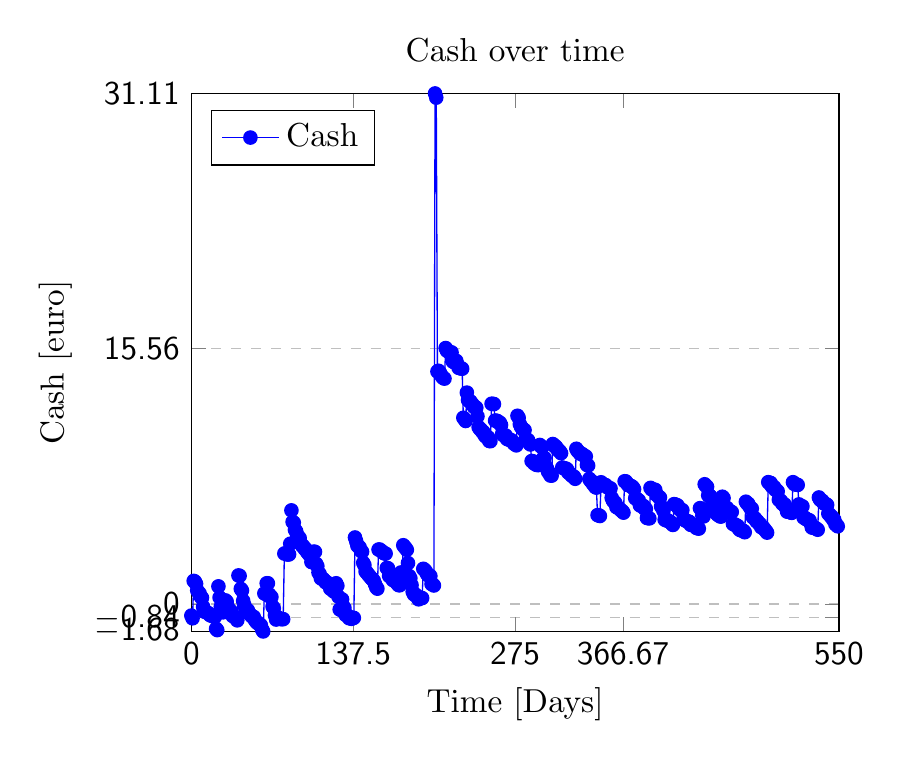
\begin{tikzpicture}[thick,scale=1.2]
\begin{axis}[
title={Cash over time},
xlabel={Time [Days]},
ylabel={Cash [euro]},
xmin=0,xmax=550,
ymin=-1.68,ymax=31.112,
xtick={0,137.5,275,366.666666666667,550},
ytick={-1.68,-0.84,0,15.556,31.112},
legend pos=north west,
ymajorgrids=true,
grid style=dashed,
]
\addplot[
color=blue,
mark=*,
]
coordinates {
(0,-0.713)(1,-0.878)(2,1.4)(3,1.36)(4,1.223)(5,0.822)(6,0.703)(7,0.636)(8,0.431)(9,0.37)(10,-0.183)(11,-0.469)(12,-0.487)(13,-0.512)(14,-0.547)(15,-0.617)(16,-0.695)(17,-0.715)(18,-0.729)(19,-0.772)(20,-0.792)(21,-1.515)(22,-1.599)(23,1.068)(24,0.388)(25,-0.181)(26,-0.339)(27,-0.515)(28,0.107)(29,0.212)(30,0.138)(31,-0.201)(32,-0.4)(33,-0.4)(34,-0.48)(35,-0.735)(36,-0.759)(37,-0.819)(38,-0.828)(39,-1.005)(40,1.734)(41,1.707)(42,0.916)(43,0.815)(44,0.187)(45,-0.071)(46,-0.325)(47,-0.361)(48,-0.384)(49,-0.595)(50,-0.639)(51,-0.739)(52,-0.794)(53,-0.794)(54,-0.988)(55,-1.084)(56,-1.164)(57,-1.189)(58,-1.239)(59,-1.299)(60,-1.553)(61,-1.68)(62,0.638)(63,0.605)(64,1.255)(65,1.255)(66,0.585)(67,0.424)(68,0.42)(69,-0.165)(70,-0.263)(71,-0.686)(72,-0.954)(73,-0.908)(74,-0.844)(75,-0.902)(76,-0.925)(77,-0.931)(78,-0.931)(79,3.069)(80,3.079)(81,3.025)(82,3.011)(83,3.016)(84,3.666)(85,5.7)(86,4.996)(87,4.947)(88,4.516)(89,4.428)(90,4.189)(91,4.069)(92,4.009)(93,3.684)(94,3.54)(95,3.52)(96,3.37)(97,3.35)(98,3.192)(99,3.112)(100,3.011)(101,2.947)(102,2.552)(103,2.537)(104,3.187)(105,3.171)(106,2.443)(107,2.297)(108,1.91)(109,1.815)(110,1.557)(111,1.541)(112,1.513)(113,1.417)(114,1.317)(115,1.317)(116,1.237)(117,1.133)(118,0.926)(119,0.914)(120,0.839)(121,0.753)(122,0.735)(123,1.256)(124,1.105)(125,0.435)(126,-0.34)(127,-0.368)(128,0.274)(129,-0.169)(130,-0.237)(131,-0.67)(132,-0.68)(133,-0.74)(134,-0.876)(135,-0.83)(136,-0.912)(137,-0.854)(138,-0.854)(139,4.046)(140,3.812)(141,3.547)(142,3.501)(143,3.44)(144,3.236)(145,3.175)(146,2.502)(147,2.358)(148,1.975)(149,1.913)(150,1.802)(151,1.726)(152,1.636)(153,1.546)(154,1.484)(155,1.404)(156,1.203)(157,1.014)(158,0.927)(159,3.312)(160,3.311)(161,3.246)(162,3.195)(163,3.115)(164,3.073)(165,3.064)(166,2.187)(167,2.171)(168,1.703)(169,1.673)(170,1.593)(171,1.461)(172,1.43)(173,1.425)(174,1.319)(175,1.226)(176,1.142)(177,1.134)(178,1.912)(179,1.902)(180,3.574)(181,3.474)(182,3.398)(183,3.292)(184,2.486)(185,1.697)(186,1.562)(187,1.147)(188,0.738)(189,0.58)(190,0.547)(191,0.529)(192,0.408)(193,0.277)(194,0.368)(195,0.353)(196,0.353)(197,2.137)(198,2.077)(199,2)(200,1.848)(201,1.747)(202,1.735)(203,1.699)(204,1.211)(205,1.193)(206,1.12)(207,31.112)(208,30.856)(209,14.164)(210,14.207)(211,14.097)(212,13.966)(213,13.837)(214,13.764)(215,13.73)(216,15.593)(217,15.433)(218,15.415)(219,15.345)(220,15.334)(221,15.329)(222,14.777)(223,14.732)(224,14.715)(225,14.814)(226,14.594)(227,14.39)(228,14.37)(229,14.353)(230,14.334)(231,11.343)(232,11.265)(233,11.148)(234,12.878)(235,12.428)(236,12.362)(237,12.342)(238,12.226)(239,12.147)(240,12.007)(241,12.002)(242,11.954)(243,11.433)(244,10.77)(245,10.665)(246,10.623)(247,10.493)(248,10.48)(249,10.285)(250,10.201)(251,10.163)(252,10.156)(253,9.929)(254,9.917)(255,12.199)(256,12.188)(257,12.18)(258,11.174)(259,11.159)(260,11.144)(261,11.052)(262,11.045)(263,10.902)(264,10.361)(265,10.277)(266,10.27)(267,10.259)(268,10.058)(269,10.029)(270,9.998)(271,9.99)(272,9.964)(273,9.875)(274,9.763)(275,9.752)(276,9.661)(277,11.465)(278,11.346)(279,10.954)(280,10.789)(281,10.714)(282,10.608)(283,10.592)(284,10.076)(285,10.004)(286,9.981)(287,9.796)(288,9.716)(289,8.705)(290,8.698)(291,8.564)(292,8.559)(293,8.472)(294,8.467)(295,8.463)(296,9.685)(297,9.59)(298,9.552)(299,8.899)(300,8.893)(301,8.362)(302,8.262)(303,8.049)(304,7.979)(305,7.824)(306,7.816)(307,9.743)(308,9.633)(309,9.623)(310,9.543)(311,9.402)(312,9.364)(313,9.291)(314,9.186)(315,8.309)(316,8.281)(317,8.255)(318,8.246)(319,8.21)(320,8.02)(321,7.965)(322,7.917)(323,7.817)(324,7.775)(325,7.751)(326,7.625)(327,9.455)(328,9.322)(329,9.276)(330,9.162)(331,9.158)(332,9.128)(333,9.064)(334,9.012)(335,8.988)(336,8.472)(337,8.429)(338,7.619)(339,7.506)(340,7.479)(341,7.316)(342,7.287)(343,7.126)(344,7.086)(345,5.41)(346,5.4)(347,5.356)(348,7.411)(349,7.285)(350,7.273)(351,7.248)(352,7.236)(353,7.13)(354,7.082)(355,7.05)(356,7.042)(357,6.468)(358,6.298)(359,6.223)(360,6.164)(361,5.899)(362,5.891)(363,5.831)(364,5.776)(365,5.694)(366,5.648)(367,5.56)(368,7.472)(369,7.464)(370,7.352)(371,7.237)(372,7.231)(373,7.187)(374,7.168)(375,7.108)(376,6.987)(377,6.438)(378,6.414)(379,6.338)(380,6.307)(381,6.003)(382,5.982)(383,5.974)(384,5.966)(385,5.797)(386,5.79)(387,5.237)(388,5.226)(389,5.21)(390,7.071)(391,6.973)(392,6.966)(393,6.959)(394,6.951)(395,6.652)(396,6.599)(397,6.509)(398,6.483)(399,5.943)(400,5.843)(401,5.67)(402,5.139)(403,5.097)(404,5.088)(405,5.076)(406,5.009)(407,4.983)(408,4.893)(409,4.811)(410,6.08)(411,6.057)(412,6.025)(413,5.995)(414,5.819)(415,5.745)(416,5.722)(417,5.715)(418,5.202)(419,5.102)(420,5.091)(421,5.024)(422,5.016)(423,5.002)(424,4.826)(425,4.805)(426,4.795)(427,4.782)(428,4.758)(429,4.627)(430,4.61)(431,4.587)(432,5.834)(433,5.794)(434,5.388)(435,5.329)(436,7.29)(437,7.2)(438,7.135)(439,6.616)(440,6.609)(441,6.541)(442,6.37)(443,5.948)(444,5.923)(445,5.584)(446,5.522)(447,5.433)(448,5.398)(449,5.33)(450,5.323)(451,6.532)(452,6.453)(453,5.904)(454,5.879)(455,5.84)(456,5.728)(457,5.62)(458,5.607)(459,5.6)(460,4.875)(461,4.838)(462,4.831)(463,4.754)(464,4.751)(465,4.575)(466,4.504)(467,4.482)(468,4.474)(469,4.451)(470,4.368)(471,6.226)(472,6.118)(473,6.1)(474,5.944)(475,5.824)(476,5.808)(477,5.27)(478,5.255)(479,5.186)(480,5.03)(481,5.023)(482,4.897)(483,4.867)(484,4.674)(485,4.65)(486,4.635)(487,4.528)(488,4.439)(489,4.342)(490,7.42)(491,7.36)(492,7.371)(493,7.162)(494,7.147)(495,7.114)(496,6.952)(497,6.927)(498,6.858)(499,6.349)(500,6.32)(501,6.252)(502,6.1)(503,6.074)(504,6.052)(505,5.87)(506,5.623)(507,5.615)(508,5.604)(509,5.575)(510,5.548)(511,7.417)(512,7.312)(513,7.29)(514,7.265)(515,7.252)(516,6.064)(517,5.958)(518,5.954)(519,5.943)(520,5.261)(521,5.253)(522,5.168)(523,5.144)(524,5.115)(525,5.093)(526,4.9)(527,4.655)(528,4.648)(529,4.639)(530,4.63)(531,4.565)(532,4.52)(533,6.485)(534,6.354)(535,6.305)(536,6.278)(537,6.141)(538,6.105)(539,6.078)(540,6.031)(541,5.502)(542,5.456)(543,5.334)(544,5.314)(545,5.144)(546,5.137)(547,4.855)(548,4.823)(549,4.728)
};
\legend{Cash}
\end{axis}
\end{tikzpicture}

\lstinputlisting[language=Octave, firstline=3, lastline=5]{../Perl/readCharges}

This is the cashCurve from perl\\
%Checklists.tex:%\includegraphics[scale=0.5]{stockchart.pdf}}

\subsubsection{Cash curve from Scilab man!}
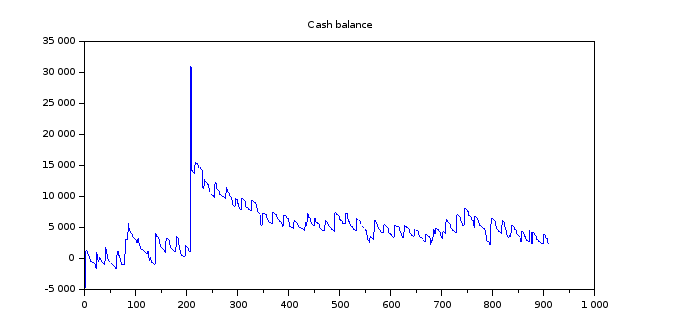
\includegraphics[scale=0.6]{Scilab-cashBalance.png}
\lstinputlisting[language=Octave, firstline=3, lastline=5]{../Perl/readCharges}

This is the cashBalance from Scilab\\

\section{Cash Balance Management}

\subsection{Monthly drift}

\subsubsection{Monthly drift table}
%\input{almGraph}
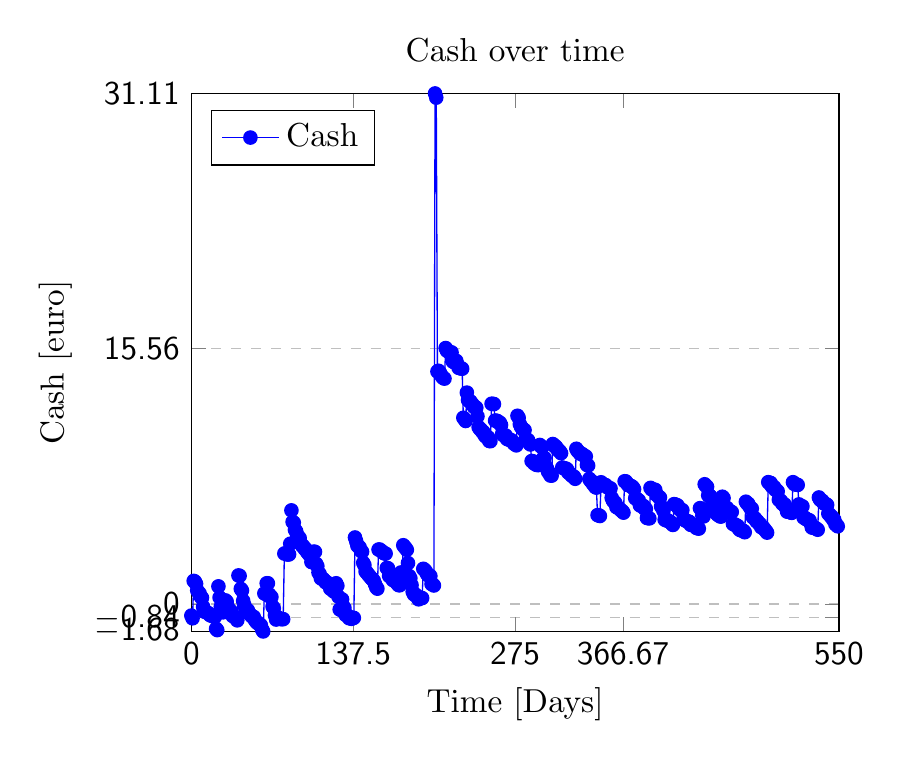
\begin{tikzpicture}[thick,scale=1.2]
\begin{axis}[
title={Cash over time},
xlabel={Time [Days]},
ylabel={Cash [euro]},
xmin=0,xmax=550,
ymin=-1.68,ymax=31.112,
xtick={0,137.5,275,366.666666666667,550},
ytick={-1.68,-0.84,0,15.556,31.112},
legend pos=north west,
ymajorgrids=true,
grid style=dashed,
]
\addplot[
color=blue,
mark=*,
]
coordinates {
(0,-0.713)(1,-0.878)(2,1.4)(3,1.36)(4,1.223)(5,0.822)(6,0.703)(7,0.636)(8,0.431)(9,0.37)(10,-0.183)(11,-0.469)(12,-0.487)(13,-0.512)(14,-0.547)(15,-0.617)(16,-0.695)(17,-0.715)(18,-0.729)(19,-0.772)(20,-0.792)(21,-1.515)(22,-1.599)(23,1.068)(24,0.388)(25,-0.181)(26,-0.339)(27,-0.515)(28,0.107)(29,0.212)(30,0.138)(31,-0.201)(32,-0.4)(33,-0.4)(34,-0.48)(35,-0.735)(36,-0.759)(37,-0.819)(38,-0.828)(39,-1.005)(40,1.734)(41,1.707)(42,0.916)(43,0.815)(44,0.187)(45,-0.071)(46,-0.325)(47,-0.361)(48,-0.384)(49,-0.595)(50,-0.639)(51,-0.739)(52,-0.794)(53,-0.794)(54,-0.988)(55,-1.084)(56,-1.164)(57,-1.189)(58,-1.239)(59,-1.299)(60,-1.553)(61,-1.68)(62,0.638)(63,0.605)(64,1.255)(65,1.255)(66,0.585)(67,0.424)(68,0.42)(69,-0.165)(70,-0.263)(71,-0.686)(72,-0.954)(73,-0.908)(74,-0.844)(75,-0.902)(76,-0.925)(77,-0.931)(78,-0.931)(79,3.069)(80,3.079)(81,3.025)(82,3.011)(83,3.016)(84,3.666)(85,5.7)(86,4.996)(87,4.947)(88,4.516)(89,4.428)(90,4.189)(91,4.069)(92,4.009)(93,3.684)(94,3.54)(95,3.52)(96,3.37)(97,3.35)(98,3.192)(99,3.112)(100,3.011)(101,2.947)(102,2.552)(103,2.537)(104,3.187)(105,3.171)(106,2.443)(107,2.297)(108,1.91)(109,1.815)(110,1.557)(111,1.541)(112,1.513)(113,1.417)(114,1.317)(115,1.317)(116,1.237)(117,1.133)(118,0.926)(119,0.914)(120,0.839)(121,0.753)(122,0.735)(123,1.256)(124,1.105)(125,0.435)(126,-0.34)(127,-0.368)(128,0.274)(129,-0.169)(130,-0.237)(131,-0.67)(132,-0.68)(133,-0.74)(134,-0.876)(135,-0.83)(136,-0.912)(137,-0.854)(138,-0.854)(139,4.046)(140,3.812)(141,3.547)(142,3.501)(143,3.44)(144,3.236)(145,3.175)(146,2.502)(147,2.358)(148,1.975)(149,1.913)(150,1.802)(151,1.726)(152,1.636)(153,1.546)(154,1.484)(155,1.404)(156,1.203)(157,1.014)(158,0.927)(159,3.312)(160,3.311)(161,3.246)(162,3.195)(163,3.115)(164,3.073)(165,3.064)(166,2.187)(167,2.171)(168,1.703)(169,1.673)(170,1.593)(171,1.461)(172,1.43)(173,1.425)(174,1.319)(175,1.226)(176,1.142)(177,1.134)(178,1.912)(179,1.902)(180,3.574)(181,3.474)(182,3.398)(183,3.292)(184,2.486)(185,1.697)(186,1.562)(187,1.147)(188,0.738)(189,0.58)(190,0.547)(191,0.529)(192,0.408)(193,0.277)(194,0.368)(195,0.353)(196,0.353)(197,2.137)(198,2.077)(199,2)(200,1.848)(201,1.747)(202,1.735)(203,1.699)(204,1.211)(205,1.193)(206,1.12)(207,31.112)(208,30.856)(209,14.164)(210,14.207)(211,14.097)(212,13.966)(213,13.837)(214,13.764)(215,13.73)(216,15.593)(217,15.433)(218,15.415)(219,15.345)(220,15.334)(221,15.329)(222,14.777)(223,14.732)(224,14.715)(225,14.814)(226,14.594)(227,14.39)(228,14.37)(229,14.353)(230,14.334)(231,11.343)(232,11.265)(233,11.148)(234,12.878)(235,12.428)(236,12.362)(237,12.342)(238,12.226)(239,12.147)(240,12.007)(241,12.002)(242,11.954)(243,11.433)(244,10.77)(245,10.665)(246,10.623)(247,10.493)(248,10.48)(249,10.285)(250,10.201)(251,10.163)(252,10.156)(253,9.929)(254,9.917)(255,12.199)(256,12.188)(257,12.18)(258,11.174)(259,11.159)(260,11.144)(261,11.052)(262,11.045)(263,10.902)(264,10.361)(265,10.277)(266,10.27)(267,10.259)(268,10.058)(269,10.029)(270,9.998)(271,9.99)(272,9.964)(273,9.875)(274,9.763)(275,9.752)(276,9.661)(277,11.465)(278,11.346)(279,10.954)(280,10.789)(281,10.714)(282,10.608)(283,10.592)(284,10.076)(285,10.004)(286,9.981)(287,9.796)(288,9.716)(289,8.705)(290,8.698)(291,8.564)(292,8.559)(293,8.472)(294,8.467)(295,8.463)(296,9.685)(297,9.59)(298,9.552)(299,8.899)(300,8.893)(301,8.362)(302,8.262)(303,8.049)(304,7.979)(305,7.824)(306,7.816)(307,9.743)(308,9.633)(309,9.623)(310,9.543)(311,9.402)(312,9.364)(313,9.291)(314,9.186)(315,8.309)(316,8.281)(317,8.255)(318,8.246)(319,8.21)(320,8.02)(321,7.965)(322,7.917)(323,7.817)(324,7.775)(325,7.751)(326,7.625)(327,9.455)(328,9.322)(329,9.276)(330,9.162)(331,9.158)(332,9.128)(333,9.064)(334,9.012)(335,8.988)(336,8.472)(337,8.429)(338,7.619)(339,7.506)(340,7.479)(341,7.316)(342,7.287)(343,7.126)(344,7.086)(345,5.41)(346,5.4)(347,5.356)(348,7.411)(349,7.285)(350,7.273)(351,7.248)(352,7.236)(353,7.13)(354,7.082)(355,7.05)(356,7.042)(357,6.468)(358,6.298)(359,6.223)(360,6.164)(361,5.899)(362,5.891)(363,5.831)(364,5.776)(365,5.694)(366,5.648)(367,5.56)(368,7.472)(369,7.464)(370,7.352)(371,7.237)(372,7.231)(373,7.187)(374,7.168)(375,7.108)(376,6.987)(377,6.438)(378,6.414)(379,6.338)(380,6.307)(381,6.003)(382,5.982)(383,5.974)(384,5.966)(385,5.797)(386,5.79)(387,5.237)(388,5.226)(389,5.21)(390,7.071)(391,6.973)(392,6.966)(393,6.959)(394,6.951)(395,6.652)(396,6.599)(397,6.509)(398,6.483)(399,5.943)(400,5.843)(401,5.67)(402,5.139)(403,5.097)(404,5.088)(405,5.076)(406,5.009)(407,4.983)(408,4.893)(409,4.811)(410,6.08)(411,6.057)(412,6.025)(413,5.995)(414,5.819)(415,5.745)(416,5.722)(417,5.715)(418,5.202)(419,5.102)(420,5.091)(421,5.024)(422,5.016)(423,5.002)(424,4.826)(425,4.805)(426,4.795)(427,4.782)(428,4.758)(429,4.627)(430,4.61)(431,4.587)(432,5.834)(433,5.794)(434,5.388)(435,5.329)(436,7.29)(437,7.2)(438,7.135)(439,6.616)(440,6.609)(441,6.541)(442,6.37)(443,5.948)(444,5.923)(445,5.584)(446,5.522)(447,5.433)(448,5.398)(449,5.33)(450,5.323)(451,6.532)(452,6.453)(453,5.904)(454,5.879)(455,5.84)(456,5.728)(457,5.62)(458,5.607)(459,5.6)(460,4.875)(461,4.838)(462,4.831)(463,4.754)(464,4.751)(465,4.575)(466,4.504)(467,4.482)(468,4.474)(469,4.451)(470,4.368)(471,6.226)(472,6.118)(473,6.1)(474,5.944)(475,5.824)(476,5.808)(477,5.27)(478,5.255)(479,5.186)(480,5.03)(481,5.023)(482,4.897)(483,4.867)(484,4.674)(485,4.65)(486,4.635)(487,4.528)(488,4.439)(489,4.342)(490,7.42)(491,7.36)(492,7.371)(493,7.162)(494,7.147)(495,7.114)(496,6.952)(497,6.927)(498,6.858)(499,6.349)(500,6.32)(501,6.252)(502,6.1)(503,6.074)(504,6.052)(505,5.87)(506,5.623)(507,5.615)(508,5.604)(509,5.575)(510,5.548)(511,7.417)(512,7.312)(513,7.29)(514,7.265)(515,7.252)(516,6.064)(517,5.958)(518,5.954)(519,5.943)(520,5.261)(521,5.253)(522,5.168)(523,5.144)(524,5.115)(525,5.093)(526,4.9)(527,4.655)(528,4.648)(529,4.639)(530,4.63)(531,4.565)(532,4.52)(533,6.485)(534,6.354)(535,6.305)(536,6.278)(537,6.141)(538,6.105)(539,6.078)(540,6.031)(541,5.502)(542,5.456)(543,5.334)(544,5.314)(545,5.144)(546,5.137)(547,4.855)(548,4.823)(549,4.728)
};
\legend{Cash}
\end{axis}
\end{tikzpicture}

\lstinputlisting[language=Octave, firstline=3, lastline=5]{../Perl/readCharges}

\subsubsection{Table of the PnL}
\begin{longtable}{|c|c|c|c|c|}
\hline
\multicolumn{5}{|c|}{Cashflows} \\
\hline
Date & Income & Charges & PnL & NumDays\\
\hline
2021-01-13 & 96890 & 92162 & 4728 & 7531\\
\hline
2017-04-20 & 96890 & 92162 & 4728 & 6167\\
\hline
2017-04-19 & 96890 & 92067 & 4823 & 6166\\
\hline
2017-04-18 & 96890 & 92035 & 4855 & 6165\\
\hline
2017-04-14 & 96890 & 91753 & 5137 & 6161\\
\hline
2017-04-13 & 96890 & 91746 & 5144 & 6160\\
\hline
2017-04-12 & 96890 & 91576 & 5314 & 6159\\
\hline
2017-04-11 & 96890 & 91556 & 5334 & 6158\\
\hline
2017-04-10 & 96890 & 91434 & 5456 & 6157\\
\hline
2017-04-07 & 96890 & 91388 & 5502 & 6154\\
\hline
2017-04-06 & 96890 & 90859 & 6031 & 6153\\
\hline
2017-04-05 & 96890 & 90812 & 6078 & 6152\\
\hline
2017-04-04 & 96890 & 90785 & 6105 & 6151\\
\hline
2017-04-03 & 96890 & 90749 & 6141 & 6150\\
\hline
2017-03-31 & 96890 & 90612 & 6278 & 6147\\
\hline
 ... & ... & ... & ... & ... & ...\\
\hline
 Total &  &  &  &  & \\
\hline
\end{longtable}

\lstinputlisting[language=Octave, firstline=3, lastline=5]{../Perl/readCharges}
There is a bug in the table that could be corrected quickly.\\
To be able to have data for the drift, you need to build a C++ insert like for the kapital
go through the dates in the cashflows, and calculate a drift based on this (modulo the salary) 
\subsubsection{Graph}
%\includegraphics[width=.8\textwidth]{PnL.png}
%\begin{bchart}[min=0,max=96,step=32,unit=k\texteuro]
\bcbar[label=Income]{96}\\
\smallskip
\bcbar[label=Charges]{92}\\
\smallskip
\bcbar[label=Drift]{4}\\
\smallskip
\bcbar[label=Income]{96}\\
\smallskip
\bcbar[label=Charges]{92}\\
\smallskip
\bcbar[label=Drift]{4}\\
\smallskip
\bcbar[label=Income]{96}\\
\smallskip
\bcbar[label=Charges]{92}\\
\smallskip
\bcbar[label=Drift]{4}\\
\smallskip
\bcbar[label=Income]{96}\\
\smallskip
\bcbar[label=Charges]{92}\\
\smallskip
\bcbar[label=Drift]{4}\\
\smallskip
\bcbar[label=Income]{96}\\
\smallskip
\bcbar[label=Charges]{91}\\
\smallskip
\bcbar[label=Drift]{5}\\
\smallskip
\bcbar[label=Income]{96}\\
\smallskip
\bcbar[label=Charges]{91}\\
\smallskip
\bcbar[label=Drift]{5}\\
\smallskip
\bcbar[label=Income]{96}\\
\smallskip
\bcbar[label=Charges]{91}\\
\smallskip
\bcbar[label=Drift]{5}\\
\smallskip
\bcbar[label=Income]{96}\\
\smallskip
\bcbar[label=Charges]{91}\\
\smallskip
\bcbar[label=Drift]{5}\\
\smallskip
\bcbar[label=Income]{96}\\
\smallskip
\bcbar[label=Charges]{91}\\
\smallskip
\bcbar[label=Drift]{5}\\
\smallskip
\bcbar[label=Income]{96}\\
\smallskip
\bcbar[label=Charges]{91}\\
\smallskip
\bcbar[label=Drift]{5}\\
\smallskip
\bcbar[label=Income]{96}\\
\smallskip
\bcbar[label=Charges]{90}\\
\smallskip
\bcbar[label=Drift]{6}\\
\smallskip
\bcbar[label=Income]{96}\\
\smallskip
\bcbar[label=Charges]{90}\\
\smallskip
\bcbar[label=Drift]{6}\\
\smallskip
\bcbar[label=Income]{96}\\
\smallskip
\bcbar[label=Charges]{90}\\
\smallskip
\bcbar[label=Drift]{6}\\
\smallskip
\bcbar[label=Income]{96}\\
\smallskip
\bcbar[label=Charges]{90}\\
\smallskip
\bcbar[label=Drift]{6}\\
\smallskip
\bcbar[label=Income]{96}\\
\smallskip
\bcbar[label=Charges]{90}\\
\smallskip
\bcbar[label=Drift]{6}\\
\smallskip
\end{bchart}

%\input{Plot}
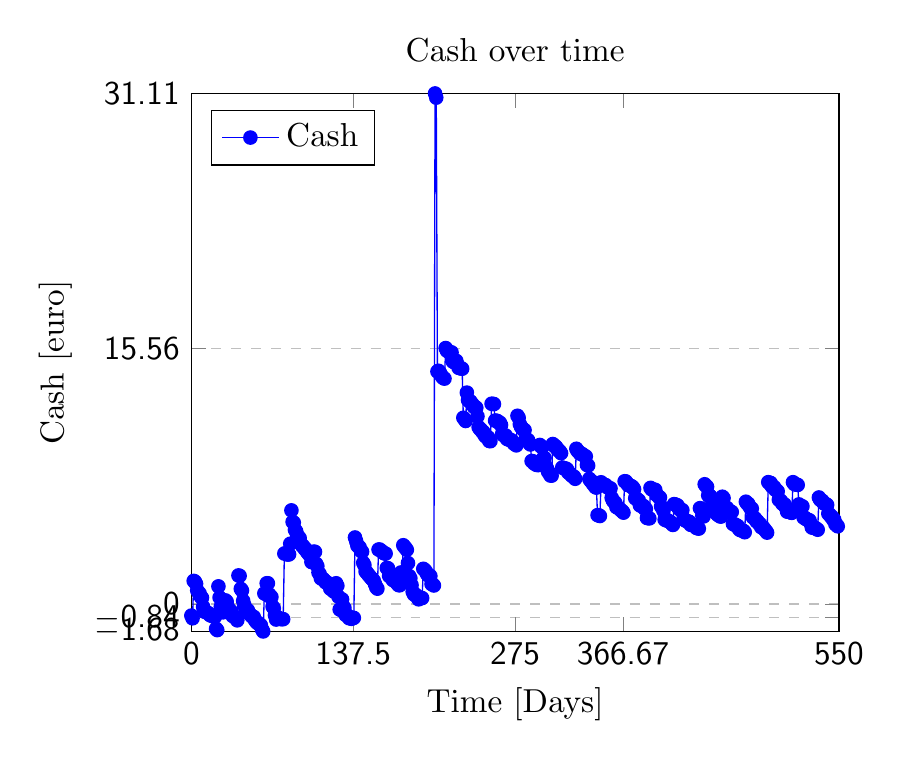
\begin{tikzpicture}[thick,scale=1.2]
\begin{axis}[
title={Cash over time},
xlabel={Time [Days]},
ylabel={Cash [euro]},
xmin=0,xmax=550,
ymin=-1.68,ymax=31.112,
xtick={0,137.5,275,366.666666666667,550},
ytick={-1.68,-0.84,0,15.556,31.112},
legend pos=north west,
ymajorgrids=true,
grid style=dashed,
]
\addplot[
color=blue,
mark=*,
]
coordinates {
(0,-0.713)(1,-0.878)(2,1.4)(3,1.36)(4,1.223)(5,0.822)(6,0.703)(7,0.636)(8,0.431)(9,0.37)(10,-0.183)(11,-0.469)(12,-0.487)(13,-0.512)(14,-0.547)(15,-0.617)(16,-0.695)(17,-0.715)(18,-0.729)(19,-0.772)(20,-0.792)(21,-1.515)(22,-1.599)(23,1.068)(24,0.388)(25,-0.181)(26,-0.339)(27,-0.515)(28,0.107)(29,0.212)(30,0.138)(31,-0.201)(32,-0.4)(33,-0.4)(34,-0.48)(35,-0.735)(36,-0.759)(37,-0.819)(38,-0.828)(39,-1.005)(40,1.734)(41,1.707)(42,0.916)(43,0.815)(44,0.187)(45,-0.071)(46,-0.325)(47,-0.361)(48,-0.384)(49,-0.595)(50,-0.639)(51,-0.739)(52,-0.794)(53,-0.794)(54,-0.988)(55,-1.084)(56,-1.164)(57,-1.189)(58,-1.239)(59,-1.299)(60,-1.553)(61,-1.68)(62,0.638)(63,0.605)(64,1.255)(65,1.255)(66,0.585)(67,0.424)(68,0.42)(69,-0.165)(70,-0.263)(71,-0.686)(72,-0.954)(73,-0.908)(74,-0.844)(75,-0.902)(76,-0.925)(77,-0.931)(78,-0.931)(79,3.069)(80,3.079)(81,3.025)(82,3.011)(83,3.016)(84,3.666)(85,5.7)(86,4.996)(87,4.947)(88,4.516)(89,4.428)(90,4.189)(91,4.069)(92,4.009)(93,3.684)(94,3.54)(95,3.52)(96,3.37)(97,3.35)(98,3.192)(99,3.112)(100,3.011)(101,2.947)(102,2.552)(103,2.537)(104,3.187)(105,3.171)(106,2.443)(107,2.297)(108,1.91)(109,1.815)(110,1.557)(111,1.541)(112,1.513)(113,1.417)(114,1.317)(115,1.317)(116,1.237)(117,1.133)(118,0.926)(119,0.914)(120,0.839)(121,0.753)(122,0.735)(123,1.256)(124,1.105)(125,0.435)(126,-0.34)(127,-0.368)(128,0.274)(129,-0.169)(130,-0.237)(131,-0.67)(132,-0.68)(133,-0.74)(134,-0.876)(135,-0.83)(136,-0.912)(137,-0.854)(138,-0.854)(139,4.046)(140,3.812)(141,3.547)(142,3.501)(143,3.44)(144,3.236)(145,3.175)(146,2.502)(147,2.358)(148,1.975)(149,1.913)(150,1.802)(151,1.726)(152,1.636)(153,1.546)(154,1.484)(155,1.404)(156,1.203)(157,1.014)(158,0.927)(159,3.312)(160,3.311)(161,3.246)(162,3.195)(163,3.115)(164,3.073)(165,3.064)(166,2.187)(167,2.171)(168,1.703)(169,1.673)(170,1.593)(171,1.461)(172,1.43)(173,1.425)(174,1.319)(175,1.226)(176,1.142)(177,1.134)(178,1.912)(179,1.902)(180,3.574)(181,3.474)(182,3.398)(183,3.292)(184,2.486)(185,1.697)(186,1.562)(187,1.147)(188,0.738)(189,0.58)(190,0.547)(191,0.529)(192,0.408)(193,0.277)(194,0.368)(195,0.353)(196,0.353)(197,2.137)(198,2.077)(199,2)(200,1.848)(201,1.747)(202,1.735)(203,1.699)(204,1.211)(205,1.193)(206,1.12)(207,31.112)(208,30.856)(209,14.164)(210,14.207)(211,14.097)(212,13.966)(213,13.837)(214,13.764)(215,13.73)(216,15.593)(217,15.433)(218,15.415)(219,15.345)(220,15.334)(221,15.329)(222,14.777)(223,14.732)(224,14.715)(225,14.814)(226,14.594)(227,14.39)(228,14.37)(229,14.353)(230,14.334)(231,11.343)(232,11.265)(233,11.148)(234,12.878)(235,12.428)(236,12.362)(237,12.342)(238,12.226)(239,12.147)(240,12.007)(241,12.002)(242,11.954)(243,11.433)(244,10.77)(245,10.665)(246,10.623)(247,10.493)(248,10.48)(249,10.285)(250,10.201)(251,10.163)(252,10.156)(253,9.929)(254,9.917)(255,12.199)(256,12.188)(257,12.18)(258,11.174)(259,11.159)(260,11.144)(261,11.052)(262,11.045)(263,10.902)(264,10.361)(265,10.277)(266,10.27)(267,10.259)(268,10.058)(269,10.029)(270,9.998)(271,9.99)(272,9.964)(273,9.875)(274,9.763)(275,9.752)(276,9.661)(277,11.465)(278,11.346)(279,10.954)(280,10.789)(281,10.714)(282,10.608)(283,10.592)(284,10.076)(285,10.004)(286,9.981)(287,9.796)(288,9.716)(289,8.705)(290,8.698)(291,8.564)(292,8.559)(293,8.472)(294,8.467)(295,8.463)(296,9.685)(297,9.59)(298,9.552)(299,8.899)(300,8.893)(301,8.362)(302,8.262)(303,8.049)(304,7.979)(305,7.824)(306,7.816)(307,9.743)(308,9.633)(309,9.623)(310,9.543)(311,9.402)(312,9.364)(313,9.291)(314,9.186)(315,8.309)(316,8.281)(317,8.255)(318,8.246)(319,8.21)(320,8.02)(321,7.965)(322,7.917)(323,7.817)(324,7.775)(325,7.751)(326,7.625)(327,9.455)(328,9.322)(329,9.276)(330,9.162)(331,9.158)(332,9.128)(333,9.064)(334,9.012)(335,8.988)(336,8.472)(337,8.429)(338,7.619)(339,7.506)(340,7.479)(341,7.316)(342,7.287)(343,7.126)(344,7.086)(345,5.41)(346,5.4)(347,5.356)(348,7.411)(349,7.285)(350,7.273)(351,7.248)(352,7.236)(353,7.13)(354,7.082)(355,7.05)(356,7.042)(357,6.468)(358,6.298)(359,6.223)(360,6.164)(361,5.899)(362,5.891)(363,5.831)(364,5.776)(365,5.694)(366,5.648)(367,5.56)(368,7.472)(369,7.464)(370,7.352)(371,7.237)(372,7.231)(373,7.187)(374,7.168)(375,7.108)(376,6.987)(377,6.438)(378,6.414)(379,6.338)(380,6.307)(381,6.003)(382,5.982)(383,5.974)(384,5.966)(385,5.797)(386,5.79)(387,5.237)(388,5.226)(389,5.21)(390,7.071)(391,6.973)(392,6.966)(393,6.959)(394,6.951)(395,6.652)(396,6.599)(397,6.509)(398,6.483)(399,5.943)(400,5.843)(401,5.67)(402,5.139)(403,5.097)(404,5.088)(405,5.076)(406,5.009)(407,4.983)(408,4.893)(409,4.811)(410,6.08)(411,6.057)(412,6.025)(413,5.995)(414,5.819)(415,5.745)(416,5.722)(417,5.715)(418,5.202)(419,5.102)(420,5.091)(421,5.024)(422,5.016)(423,5.002)(424,4.826)(425,4.805)(426,4.795)(427,4.782)(428,4.758)(429,4.627)(430,4.61)(431,4.587)(432,5.834)(433,5.794)(434,5.388)(435,5.329)(436,7.29)(437,7.2)(438,7.135)(439,6.616)(440,6.609)(441,6.541)(442,6.37)(443,5.948)(444,5.923)(445,5.584)(446,5.522)(447,5.433)(448,5.398)(449,5.33)(450,5.323)(451,6.532)(452,6.453)(453,5.904)(454,5.879)(455,5.84)(456,5.728)(457,5.62)(458,5.607)(459,5.6)(460,4.875)(461,4.838)(462,4.831)(463,4.754)(464,4.751)(465,4.575)(466,4.504)(467,4.482)(468,4.474)(469,4.451)(470,4.368)(471,6.226)(472,6.118)(473,6.1)(474,5.944)(475,5.824)(476,5.808)(477,5.27)(478,5.255)(479,5.186)(480,5.03)(481,5.023)(482,4.897)(483,4.867)(484,4.674)(485,4.65)(486,4.635)(487,4.528)(488,4.439)(489,4.342)(490,7.42)(491,7.36)(492,7.371)(493,7.162)(494,7.147)(495,7.114)(496,6.952)(497,6.927)(498,6.858)(499,6.349)(500,6.32)(501,6.252)(502,6.1)(503,6.074)(504,6.052)(505,5.87)(506,5.623)(507,5.615)(508,5.604)(509,5.575)(510,5.548)(511,7.417)(512,7.312)(513,7.29)(514,7.265)(515,7.252)(516,6.064)(517,5.958)(518,5.954)(519,5.943)(520,5.261)(521,5.253)(522,5.168)(523,5.144)(524,5.115)(525,5.093)(526,4.9)(527,4.655)(528,4.648)(529,4.639)(530,4.63)(531,4.565)(532,4.52)(533,6.485)(534,6.354)(535,6.305)(536,6.278)(537,6.141)(538,6.105)(539,6.078)(540,6.031)(541,5.502)(542,5.456)(543,5.334)(544,5.314)(545,5.144)(546,5.137)(547,4.855)(548,4.823)(549,4.728)
};
\legend{Cash}
\end{axis}
\end{tikzpicture}

\lstinputlisting[language=Octave, firstline=3, lastline=5]{../Perl/readCharges}
\subsection{Incomes}
%Data are aggregated between Initial date: \textbf{2000-01-01} and Last date: \textbf{2018-11-16 00:00:00}


\subsubsection{Income table}
\begin{longtable}{|c|c|c|c|c|}
\hline
\multicolumn{5}{|c|}{Cashflows} \\
\hline
Category & Debit & Credit & PnL \\
\hline
Salary & 0 & 86580 & 86580\\
\hline
Funding & 0 & 42600 & 42600\\
\hline
Cmb & 0 & 7287 & 7287\\
\hline
Bank & 0 & 6097 & 6097\\
\hline
Debt & 0 & 2549 & 2549\\
\hline
Taxes & 0 & 1824 & 1824\\
\hline
Other & 0 & 1191 & 1191\\
\hline
Rent & 0 & 149 & 149\\
\hline
Telephone & 0 & 128 & 128\\
\hline
 ... & ... & ...\\
\hline
 Total & 140420 & 142872 & 2452 \\
\hline
\end{longtable}

\lstinputlisting[language=Octave, firstline=3, lastline=5]{../Perl/readCharges}
\subsubsection{Income graph}
\begin{bchart}[min=0,max=86,step=17,unit=k\texteuro]
\bcbar[label=Salary]{86}\\
\smallskip
\bcbar[label=Funding]{42}\\
\smallskip
\bcbar[label=Cmb]{7}\\
\smallskip
\bcbar[label=Bank]{6}\\
\smallskip
\bcbar[label=Debt]{2}\\
\smallskip
\bcbar[label=Taxes]{1}\\
\smallskip
\bcbar[label=Other]{1}\\
\smallskip
\bcbar[label=Rent]{0}\\
\smallskip
\bcbar[label=Telephone]{0}\\
\smallskip
\end{bchart}

\lstinputlisting[language=Octave, firstline=3, lastline=5]{../Perl/readCharges}
\subsubsection{Income Chart}
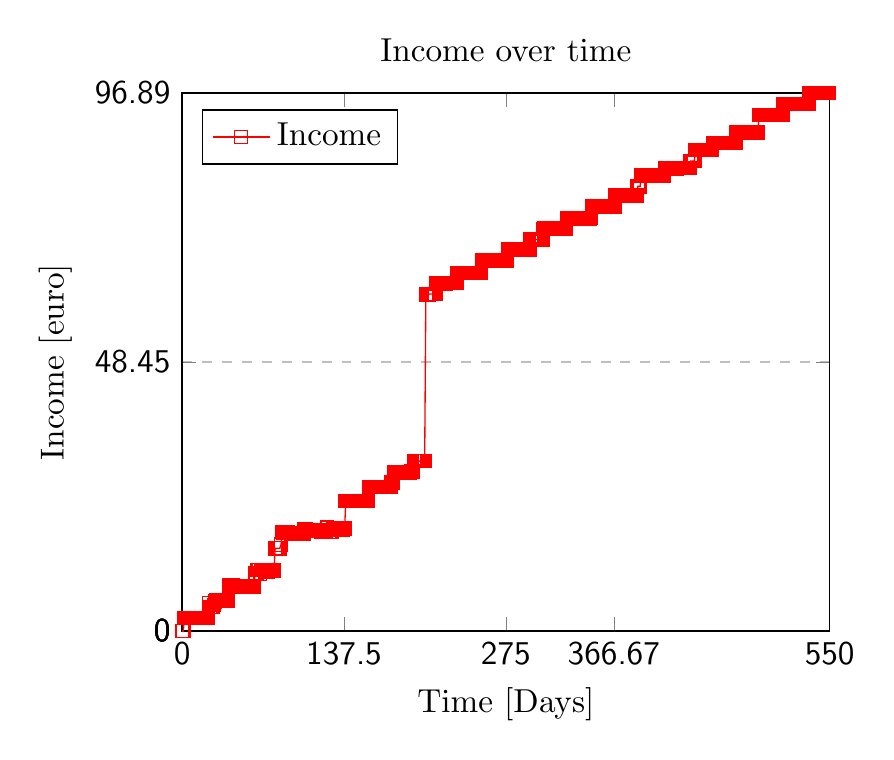
\begin{tikzpicture}[thick, scale=1.2]
\begin{axis}[
title={Income over time},
xlabel={Time [Days]},
ylabel={Income [euro]},
xmin=0,xmax=550,
ymin=0,ymax=96.89,
xtick={0,137.5,275,366.666666666667,550},
ytick={0,0,0,48.445,96.89},
legend pos=north west,
ymajorgrids=true,
grid style=dashed,
]
\addplot[
color=red,
mark=square,
]
coordinates {
(0,0)(1,0)(2,2.34)(3,2.34)(4,2.34)(5,2.34)(6,2.34)(7,2.34)(8,2.34)(9,2.34)(10,2.34)(11,2.34)(12,2.34)(13,2.34)(14,2.34)(15,2.34)(16,2.34)(17,2.34)(18,2.34)(19,2.34)(20,2.34)(21,2.34)(22,2.34)(23,5.015)(24,4.345)(25,4.345)(26,4.345)(27,4.68)(28,5.38)(29,5.485)(30,5.485)(31,5.485)(32,5.485)(33,5.485)(34,5.485)(35,5.485)(36,5.485)(37,5.485)(38,5.485)(39,5.485)(40,8.248)(41,8.248)(42,8.228)(43,8.228)(44,8.102)(45,8.112)(46,8.112)(47,8.112)(48,8.112)(49,8.002)(50,8.01)(51,8.026)(52,8.034)(53,8.034)(54,7.925)(55,7.941)(56,7.957)(57,7.965)(58,7.981)(59,7.981)(60,7.981)(61,8.005)(62,10.345)(63,10.345)(64,10.995)(65,10.995)(66,10.325)(67,10.975)(68,10.975)(69,10.975)(70,10.975)(71,10.724)(72,10.621)(73,10.713)(74,10.803)(75,10.865)(76,10.865)(77,10.881)(78,10.889)(79,14.889)(80,14.899)(81,14.91)(82,14.91)(83,14.916)(84,15.566)(85,17.83)(86,17.81)(87,17.81)(88,17.81)(89,17.81)(90,17.81)(91,17.7)(92,17.7)(93,17.596)(94,17.596)(95,17.596)(96,17.596)(97,17.596)(98,17.596)(99,17.596)(100,17.596)(101,17.596)(102,17.596)(103,17.596)(104,18.246)(105,18.246)(106,18.226)(107,18.226)(108,18.226)(109,18.226)(110,18.116)(111,18.116)(112,18.116)(113,18.116)(114,18.116)(115,18.116)(116,18.116)(117,18.116)(118,17.99)(119,17.99)(120,17.99)(121,17.99)(122,17.99)(123,18.64)(124,18.497)(125,17.827)(126,17.827)(127,17.827)(128,18.477)(129,18.477)(130,18.477)(131,18.264)(132,18.28)(133,18.28)(134,18.288)(135,18.334)(136,18.342)(137,18.44)(138,18.448)(139,23.448)(140,23.448)(141,23.448)(142,23.448)(143,23.448)(144,23.448)(145,23.448)(146,23.448)(147,23.448)(148,23.448)(149,23.448)(150,23.448)(151,23.448)(152,23.448)(153,23.448)(154,23.448)(155,23.448)(156,23.448)(157,23.448)(158,23.448)(159,25.937)(160,25.937)(161,25.937)(162,25.937)(163,25.937)(164,25.937)(165,25.937)(166,25.937)(167,25.937)(168,25.937)(169,25.937)(170,25.937)(171,25.937)(172,25.937)(173,25.937)(174,25.937)(175,25.937)(176,25.937)(177,25.937)(178,26.737)(179,26.737)(180,28.562)(181,28.562)(182,28.562)(183,28.562)(184,28.562)(185,28.562)(186,28.562)(187,28.562)(188,28.562)(189,28.562)(190,28.562)(191,28.562)(192,28.562)(193,28.565)(194,28.685)(195,28.693)(196,28.709)(197,30.605)(198,30.605)(199,30.605)(200,30.605)(201,30.605)(202,30.605)(203,30.605)(204,30.605)(205,30.605)(206,30.605)(207,60.605)(208,60.605)(209,60.605)(210,60.704)(211,60.704)(212,60.704)(213,60.704)(214,60.704)(215,60.704)(216,62.595)(217,62.6)(218,62.6)(219,62.6)(220,62.6)(221,62.6)(222,62.6)(223,62.6)(224,62.6)(225,62.704)(226,62.704)(227,62.704)(228,62.704)(229,62.704)(230,62.704)(231,62.704)(232,62.704)(233,62.704)(234,64.462)(235,64.462)(236,64.462)(237,64.462)(238,64.462)(239,64.462)(240,64.462)(241,64.462)(242,64.462)(243,64.462)(244,64.462)(245,64.462)(246,64.462)(247,64.462)(248,64.462)(249,64.462)(250,64.462)(251,64.462)(252,64.462)(253,64.462)(254,64.462)(255,66.774)(256,66.774)(257,66.774)(258,66.774)(259,66.774)(260,66.774)(261,66.774)(262,66.774)(263,66.774)(264,66.774)(265,66.774)(266,66.774)(267,66.774)(268,66.774)(269,66.774)(270,66.774)(271,66.774)(272,66.774)(273,66.774)(274,66.774)(275,66.787)(276,66.787)(277,68.729)(278,68.729)(279,68.729)(280,68.729)(281,68.729)(282,68.729)(283,68.729)(284,68.729)(285,68.729)(286,68.729)(287,68.729)(288,68.729)(289,68.729)(290,68.729)(291,68.729)(292,68.729)(293,68.729)(294,68.729)(295,68.729)(296,70.516)(297,70.516)(298,70.516)(299,70.516)(300,70.516)(301,70.516)(302,70.516)(303,70.516)(304,70.516)(305,70.516)(306,70.516)(307,72.443)(308,72.468)(309,72.468)(310,72.468)(311,72.468)(312,72.488)(313,72.488)(314,72.488)(315,72.488)(316,72.488)(317,72.488)(318,72.488)(319,72.488)(320,72.488)(321,72.488)(322,72.488)(323,72.488)(324,72.488)(325,72.488)(326,72.488)(327,74.347)(328,74.347)(329,74.347)(330,74.347)(331,74.347)(332,74.347)(333,74.347)(334,74.347)(335,74.347)(336,74.347)(337,74.347)(338,74.347)(339,74.347)(340,74.347)(341,74.347)(342,74.347)(343,74.347)(344,74.347)(345,74.347)(346,74.347)(347,74.359)(348,76.486)(349,76.486)(350,76.486)(351,76.486)(352,76.486)(353,76.486)(354,76.486)(355,76.486)(356,76.486)(357,76.486)(358,76.486)(359,76.486)(360,76.486)(361,76.486)(362,76.486)(363,76.486)(364,76.486)(365,76.486)(366,76.486)(367,76.486)(368,78.405)(369,78.42)(370,78.42)(371,78.42)(372,78.42)(373,78.42)(374,78.42)(375,78.42)(376,78.42)(377,78.42)(378,78.42)(379,78.42)(380,78.42)(381,78.42)(382,78.42)(383,78.42)(384,78.42)(385,78.42)(386,78.42)(387,80.09)(388,80.09)(389,80.09)(390,82.027)(391,82.027)(392,82.027)(393,82.027)(394,82.027)(395,82.027)(396,82.027)(397,82.027)(398,82.027)(399,82.027)(400,82.027)(401,82.027)(402,82.027)(403,82.027)(404,82.027)(405,82.027)(406,82.027)(407,82.027)(408,82.027)(409,82.027)(410,83.303)(411,83.303)(412,83.303)(413,83.303)(414,83.303)(415,83.303)(416,83.303)(417,83.303)(418,83.303)(419,83.303)(420,83.303)(421,83.38)(422,83.38)(423,83.38)(424,83.38)(425,83.38)(426,83.38)(427,83.38)(428,83.38)(429,83.38)(430,83.38)(431,83.38)(432,84.631)(433,84.631)(434,84.631)(435,84.631)(436,86.631)(437,86.631)(438,86.631)(439,86.631)(440,86.631)(441,86.631)(442,86.631)(443,86.631)(444,86.631)(445,86.631)(446,86.631)(447,86.631)(448,86.631)(449,86.631)(450,86.631)(451,87.888)(452,87.888)(453,87.888)(454,87.888)(455,87.888)(456,87.888)(457,87.888)(458,87.888)(459,87.888)(460,87.888)(461,87.888)(462,87.888)(463,87.888)(464,87.888)(465,87.888)(466,87.888)(467,87.888)(468,87.888)(469,87.888)(470,87.888)(471,89.814)(472,89.814)(473,89.814)(474,89.814)(475,89.814)(476,89.814)(477,89.814)(478,89.814)(479,89.814)(480,89.814)(481,89.814)(482,89.814)(483,89.814)(484,89.814)(485,89.814)(486,89.814)(487,89.814)(488,89.814)(489,89.814)(490,92.943)(491,92.943)(492,92.958)(493,92.958)(494,92.958)(495,92.958)(496,92.958)(497,92.958)(498,92.958)(499,92.958)(500,92.958)(501,92.958)(502,92.958)(503,92.958)(504,92.958)(505,92.958)(506,92.958)(507,92.958)(508,92.958)(509,92.958)(510,92.958)(511,94.89)(512,94.89)(513,94.89)(514,94.89)(515,94.89)(516,94.89)(517,94.89)(518,94.89)(519,94.89)(520,94.89)(521,94.89)(522,94.89)(523,94.89)(524,94.89)(525,94.89)(526,94.89)(527,94.89)(528,94.89)(529,94.89)(530,94.89)(531,94.89)(532,94.89)(533,96.89)(534,96.89)(535,96.89)(536,96.89)(537,96.89)(538,96.89)(539,96.89)(540,96.89)(541,96.89)(542,96.89)(543,96.89)(544,96.89)(545,96.89)(546,96.89)(547,96.89)(548,96.89)(549,96.89)
};
\legend{Income}
\end{axis}
\end{tikzpicture}

\lstinputlisting[language=Octave, firstline=3, lastline=5]{../Perl/readCharges}
There should be the period as for all the other graphs...\\
%\includegraphics[width=.8\textwidth]{Income.png}

\subsection{Charges}
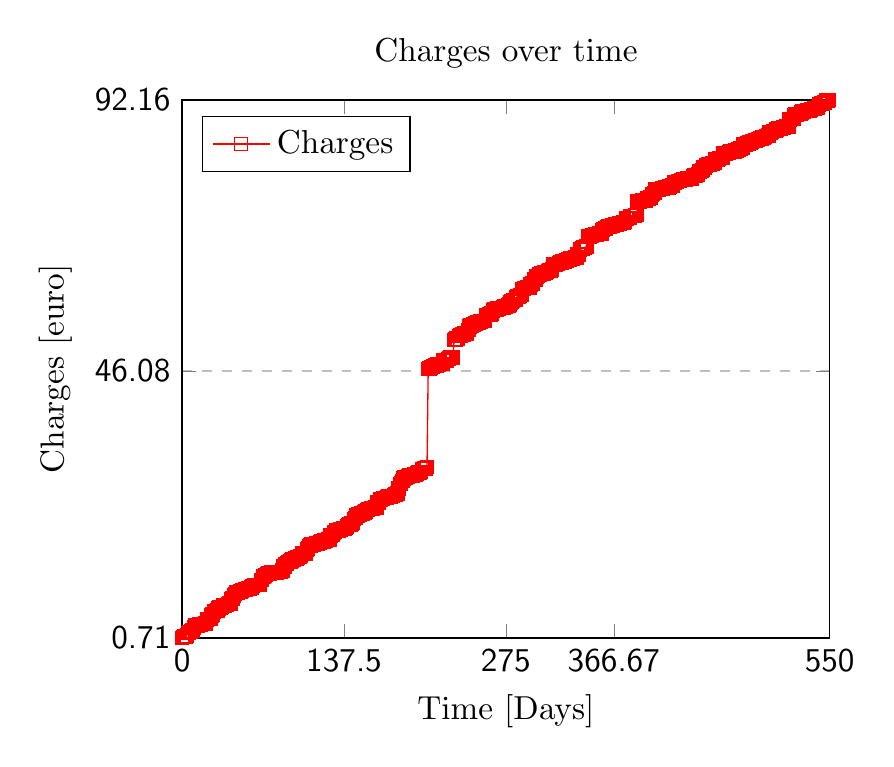
\begin{tikzpicture}[thick, scale=1.2]
\begin{axis}[
title={Charges over time},
xlabel={Time [Days]},
ylabel={Charges [euro]},
xmin=0,xmax=550,
ymin=0.713,ymax=92.162,
xtick={0,137.5,275,366.666666666667,550},
ytick={0.713,0.3565,0,46.081,92.162},
legend pos=north west,
ymajorgrids=true,
grid style=dashed,
]
\addplot[
color=red,
mark=square,
]
coordinates {
(0,0.713)(1,0.878)(2,0.94)(3,0.98)(4,1.117)(5,1.518)(6,1.637)(7,1.704)(8,1.909)(9,1.97)(10,2.523)(11,2.809)(12,2.827)(13,2.852)(14,2.887)(15,2.957)(16,3.035)(17,3.055)(18,3.069)(19,3.112)(20,3.132)(21,3.855)(22,3.939)(23,3.947)(24,3.957)(25,4.526)(26,4.684)(27,5.195)(28,5.273)(29,5.273)(30,5.347)(31,5.686)(32,5.885)(33,5.885)(34,5.965)(35,6.22)(36,6.244)(37,6.304)(38,6.313)(39,6.49)(40,6.514)(41,6.541)(42,7.312)(43,7.413)(44,7.915)(45,8.183)(46,8.437)(47,8.473)(48,8.496)(49,8.597)(50,8.649)(51,8.765)(52,8.828)(53,8.828)(54,8.913)(55,9.025)(56,9.121)(57,9.154)(58,9.22)(59,9.28)(60,9.534)(61,9.685)(62,9.707)(63,9.74)(64,9.74)(65,9.74)(66,9.74)(67,10.551)(68,10.555)(69,11.14)(70,11.238)(71,11.41)(72,11.575)(73,11.621)(74,11.647)(75,11.767)(76,11.79)(77,11.812)(78,11.82)(79,11.82)(80,11.82)(81,11.885)(82,11.899)(83,11.9)(84,11.9)(85,12.13)(86,12.814)(87,12.863)(88,13.294)(89,13.382)(90,13.621)(91,13.631)(92,13.691)(93,13.912)(94,14.056)(95,14.076)(96,14.226)(97,14.246)(98,14.404)(99,14.484)(100,14.585)(101,14.649)(102,15.044)(103,15.059)(104,15.059)(105,15.075)(106,15.783)(107,15.929)(108,16.316)(109,16.411)(110,16.559)(111,16.575)(112,16.603)(113,16.699)(114,16.799)(115,16.799)(116,16.879)(117,16.983)(118,17.064)(119,17.076)(120,17.151)(121,17.237)(122,17.255)(123,17.384)(124,17.392)(125,17.392)(126,18.167)(127,18.195)(128,18.203)(129,18.646)(130,18.714)(131,18.934)(132,18.96)(133,19.02)(134,19.164)(135,19.164)(136,19.254)(137,19.294)(138,19.302)(139,19.402)(140,19.636)(141,19.901)(142,19.947)(143,20.008)(144,20.212)(145,20.273)(146,20.946)(147,21.09)(148,21.473)(149,21.535)(150,21.646)(151,21.722)(152,21.812)(153,21.902)(154,21.964)(155,22.044)(156,22.245)(157,22.434)(158,22.521)(159,22.625)(160,22.626)(161,22.691)(162,22.742)(163,22.822)(164,22.864)(165,22.873)(166,23.75)(167,23.766)(168,24.234)(169,24.264)(170,24.344)(171,24.476)(172,24.507)(173,24.512)(174,24.618)(175,24.711)(176,24.795)(177,24.803)(178,24.825)(179,24.835)(180,24.988)(181,25.088)(182,25.164)(183,25.27)(184,26.076)(185,26.865)(186,27)(187,27.415)(188,27.824)(189,27.982)(190,28.015)(191,28.033)(192,28.154)(193,28.288)(194,28.317)(195,28.34)(196,28.356)(197,28.468)(198,28.528)(199,28.605)(200,28.757)(201,28.858)(202,28.87)(203,28.906)(204,29.394)(205,29.412)(206,29.485)(207,29.493)(208,29.749)(209,46.441)(210,46.497)(211,46.607)(212,46.738)(213,46.867)(214,46.94)(215,46.974)(216,47.002)(217,47.167)(218,47.185)(219,47.255)(220,47.266)(221,47.271)(222,47.823)(223,47.868)(224,47.885)(225,47.89)(226,48.11)(227,48.314)(228,48.334)(229,48.351)(230,48.37)(231,51.361)(232,51.439)(233,51.556)(234,51.584)(235,52.034)(236,52.1)(237,52.12)(238,52.236)(239,52.315)(240,52.455)(241,52.46)(242,52.508)(243,53.029)(244,53.692)(245,53.797)(246,53.839)(247,53.969)(248,53.982)(249,54.177)(250,54.261)(251,54.299)(252,54.306)(253,54.533)(254,54.545)(255,54.575)(256,54.586)(257,54.594)(258,55.6)(259,55.615)(260,55.63)(261,55.722)(262,55.729)(263,55.872)(264,56.413)(265,56.497)(266,56.504)(267,56.515)(268,56.716)(269,56.745)(270,56.776)(271,56.784)(272,56.81)(273,56.899)(274,57.011)(275,57.035)(276,57.126)(277,57.264)(278,57.383)(279,57.775)(280,57.94)(281,58.015)(282,58.121)(283,58.137)(284,58.653)(285,58.725)(286,58.748)(287,58.933)(288,59.013)(289,60.024)(290,60.031)(291,60.165)(292,60.17)(293,60.257)(294,60.262)(295,60.266)(296,60.831)(297,60.926)(298,60.964)(299,61.617)(300,61.623)(301,62.154)(302,62.254)(303,62.467)(304,62.537)(305,62.692)(306,62.7)(307,62.7)(308,62.835)(309,62.845)(310,62.925)(311,63.066)(312,63.124)(313,63.197)(314,63.302)(315,64.179)(316,64.207)(317,64.233)(318,64.242)(319,64.278)(320,64.468)(321,64.523)(322,64.571)(323,64.671)(324,64.713)(325,64.737)(326,64.863)(327,64.892)(328,65.025)(329,65.071)(330,65.185)(331,65.189)(332,65.219)(333,65.283)(334,65.335)(335,65.359)(336,65.875)(337,65.918)(338,66.728)(339,66.841)(340,66.868)(341,67.031)(342,67.06)(343,67.221)(344,67.261)(345,68.937)(346,68.947)(347,69.003)(348,69.075)(349,69.201)(350,69.213)(351,69.238)(352,69.25)(353,69.356)(354,69.404)(355,69.436)(356,69.444)(357,70.018)(358,70.188)(359,70.263)(360,70.322)(361,70.587)(362,70.595)(363,70.655)(364,70.71)(365,70.792)(366,70.838)(367,70.926)(368,70.933)(369,70.956)(370,71.068)(371,71.183)(372,71.189)(373,71.233)(374,71.252)(375,71.312)(376,71.433)(377,71.982)(378,72.006)(379,72.082)(380,72.113)(381,72.417)(382,72.438)(383,72.446)(384,72.454)(385,72.623)(386,72.63)(387,74.853)(388,74.864)(389,74.88)(390,74.956)(391,75.054)(392,75.061)(393,75.068)(394,75.076)(395,75.375)(396,75.428)(397,75.518)(398,75.544)(399,76.084)(400,76.184)(401,76.357)(402,76.888)(403,76.93)(404,76.939)(405,76.951)(406,77.018)(407,77.044)(408,77.134)(409,77.216)(410,77.223)(411,77.246)(412,77.278)(413,77.308)(414,77.484)(415,77.558)(416,77.581)(417,77.588)(418,78.101)(419,78.201)(420,78.212)(421,78.356)(422,78.364)(423,78.378)(424,78.554)(425,78.575)(426,78.585)(427,78.598)(428,78.622)(429,78.753)(430,78.77)(431,78.793)(432,78.797)(433,78.837)(434,79.243)(435,79.302)(436,79.341)(437,79.431)(438,79.496)(439,80.015)(440,80.022)(441,80.09)(442,80.261)(443,80.683)(444,80.708)(445,81.047)(446,81.109)(447,81.198)(448,81.233)(449,81.301)(450,81.308)(451,81.356)(452,81.435)(453,81.984)(454,82.009)(455,82.048)(456,82.16)(457,82.268)(458,82.281)(459,82.288)(460,83.013)(461,83.05)(462,83.057)(463,83.134)(464,83.137)(465,83.313)(466,83.384)(467,83.406)(468,83.414)(469,83.437)(470,83.52)(471,83.588)(472,83.696)(473,83.714)(474,83.87)(475,83.99)(476,84.006)(477,84.544)(478,84.559)(479,84.628)(480,84.784)(481,84.791)(482,84.917)(483,84.947)(484,85.14)(485,85.164)(486,85.179)(487,85.286)(488,85.375)(489,85.472)(490,85.523)(491,85.583)(492,85.587)(493,85.796)(494,85.811)(495,85.844)(496,86.006)(497,86.031)(498,86.1)(499,86.609)(500,86.638)(501,86.706)(502,86.858)(503,86.884)(504,86.906)(505,87.088)(506,87.335)(507,87.343)(508,87.354)(509,87.383)(510,87.41)(511,87.473)(512,87.578)(513,87.6)(514,87.625)(515,87.638)(516,88.826)(517,88.932)(518,88.936)(519,88.947)(520,89.629)(521,89.637)(522,89.722)(523,89.746)(524,89.775)(525,89.797)(526,89.99)(527,90.235)(528,90.242)(529,90.251)(530,90.26)(531,90.325)(532,90.37)(533,90.405)(534,90.536)(535,90.585)(536,90.612)(537,90.749)(538,90.785)(539,90.812)(540,90.859)(541,91.388)(542,91.434)(543,91.556)(544,91.576)(545,91.746)(546,91.753)(547,92.035)(548,92.067)(549,92.162)
};
\legend{Charges}
\end{axis}
\end{tikzpicture}

\lstinputlisting[language=Octave, firstline=3, lastline=5]{../Perl/readCharges}
There should be the period as for all the other graphs...\\

\subsubsection{Charges plot}
%Removed to preserve my eyes from the colors....!!!!\\
\includegraphics[scale=0.45]{Charges.png}
\lstinputlisting[language=Octave, firstline=3, lastline=5]{../Perl/readCharges}
It would be interesting to understand the period used to draw this graph.\\
There should be the period as for all the other graphs...\\

\subsubsection{Charges Scilab}
%Removed to preserve my eyes from the colors....!!!!\\
\begin{figure}
\begin{center}
%\centerline{\includegraphics[scale=0.8]{../Maths/Scilab-categories.png}}
\includegraphics[scale=0.8]{../Maths/Scilab-categories.png}
\lstinputlisting[language=Octave, firstline=3, lastline=5]{../Perl/readCharges}
\end{center}
\end{figure}

\subsubsection{Charges kiviat}
%One note :-) This should be random!
\input{chargesKiviat}
\lstinputlisting[language=Octave, firstline=3, lastline=5]{../Perl/readCharges}
There should be the period as for all the other graphs...\\

\subsubsection{Table}
\begin{longtable}{|c|c|c|c|c|}
\hline
\multicolumn{5}{|c|}{Cashflows} \\
\hline
Category & Debit & Credit & PnL \\
\hline
Cmb & 6866 & -963 & -7829\\
\hline
Debt & 25532 & 0 & -25532\\
\hline
Food & 19400 & 0 & -19400\\
\hline
Swap & 16683 & 0 & -16683\\
\hline
Other & 13685 & 0 & -13685\\
\hline
Toxics & 13497 & 0 & -13497\\
\hline
Cash & 12936 & 0 & -12936\\
\hline
Bank & 6625 & 0 & -6625\\
\hline
Rent & 5785 & 0 & -5785\\
\hline
Taxes & 4177 & 0 & -4177\\
\hline
Port & 3481 & 0 & -3481\\
\hline
Funding & 2700 & 0 & -2700\\
\hline
Telephone & 2357 & 0 & -2357\\
\hline
Health & 1505 & 0 & -1505\\
\hline
Investments & 1188 & 0 & -1188\\
\hline
Transport & 1166 & 0 & -1166\\
\hline
Car & 988 & 0 & -988\\
\hline
Energy & 568 & 0 & -568\\
\hline
Home & 519 & 0 & -519\\
\hline
Boat & 408 & 0 & -408\\
\hline
Crooks & 249 & 0 & -249\\
\hline
Presents & 105 & 0 & -105\\
\hline
 ... & ... & ... & ...\\
\hline
 Total & 140420 & 142872 & 2452 \\
\hline
\end{longtable}

\lstinputlisting[language=Octave, firstline=3, lastline=5]{../Perl/readCharges}

\subsubsection{Graph}
\begin{bchart}[min=0,max=25,step=5,unit=k\texteuro]
\bcbar[label=Cmb]{6}\\
\smallskip
\bcbar[label=Debt]{25}\\
\smallskip
\bcbar[label=Food]{19}\\
\smallskip
\bcbar[label=Swap]{16}\\
\smallskip
\bcbar[label=Other]{13}\\
\smallskip
\bcbar[label=Toxics]{13}\\
\smallskip
\bcbar[label=Cash]{12}\\
\smallskip
\bcbar[label=Bank]{6}\\
\smallskip
\bcbar[label=Rent]{5}\\
\smallskip
\bcbar[label=Taxes]{4}\\
\smallskip
\bcbar[label=Port]{3}\\
\smallskip
\bcbar[label=Funding]{2}\\
\smallskip
\bcbar[label=Telephone]{2}\\
\smallskip
\bcbar[label=Health]{1}\\
\smallskip
\bcbar[label=Investments]{1}\\
\smallskip
\bcbar[label=Transport]{1}\\
\smallskip
\bcbar[label=Car]{0}\\
\smallskip
\bcbar[label=Energy]{0}\\
\smallskip
\bcbar[label=Home]{0}\\
\smallskip
\bcbar[label=Boat]{0}\\
\smallskip
\bcbar[label=Crooks]{0}\\
\smallskip
\bcbar[label=Presents]{0}\\
\smallskip
\end{bchart}

\lstinputlisting[language=Octave, firstline=3, lastline=5]{../Perl/readCharges}
There should be the period as for all the other graphs...\\

\subsubsection{Chart}
What are we supposed to see here?!\\

\subsubsection{Cheese}
\begin{tikzpicture}[scale=2]
\foreach \p/\t in {
4 / Cmb-6.866k\texteuro ,
18 / Debt-25.532k\texteuro ,
13 / Food-19.4k\texteuro ,
11 / Swap-16.683k\texteuro ,
9 / Other-13.685k\texteuro ,
9 / Toxics-13.497k\texteuro ,
9 / Cash-12.936k\texteuro ,
4 / Bank-6.625k\texteuro ,
4 / Rent-5.785k\texteuro ,
2 / Taxes-4.177k\texteuro ,
2 / Port-3.481k\texteuro ,
1 / Funding-2.7k\texteuro ,
1 / Telephone-2.357k\texteuro ,
1 / Health-1.505k\texteuro ,
0 / Investments-1.188k\texteuro ,
0 / Transport-1.166k\texteuro ,
0 / Car-0.988k\texteuro ,
0 / Energy-0.568k\texteuro ,
0 / Home-0.519k\texteuro ,
0 / Boat-0.408k\texteuro ,
0 / Crooks-0.249k\texteuro ,
0 / Presents-0.105k\texteuro ,
}
  {
\setcounter{a}{\value{b}}
\addtocounter{b}{\p}
\slice{\thea/100*360}
          {\theb/100*360}
          {\p\%}{\t}
  }
\end{tikzpicture}

\lstinputlisting[language=Octave, firstline=3, lastline=5]{../Perl/readCharges}
Here there are a couple of changes that need to be made, starting from the colors of the graph.\\
\section{Asset Liability Management}

\subsection{Kapital}

\subsubsection{Table}
History of the Kapital is available in the database (select * from kapital)\\
Where is the table?!\\

%$\lim_{x \to \infty} \exp(-x) = 0$
%$\lim_{x \to \infty} \exp(-x) = 0$
%K: Kapital\\
%A: Assets\\
%L: Liabilities\\
%K = A-L\\
%L = K/L\\

\subsubsection{Graph}
A graph of the kapital and not income and charges cumulated should be easy to build.
Say a readKapital which would select the cash balance + all the other stuff like assets - liabilities
Better do it with Latex than with the C++ 

\subsubsection{History}
{\footnotesize
Historical graph of the kapital, liab and assets, yearly ALM management\\
%\includegraphics[width=.8\textwidth]{Assets.png}
}

\subsubsection{Definitions}
{\footnotesize
Vp: value weight (basically the value of the asset against the total value - to be replaced by InitPrice)\\
Rp: return weight (the return compared to the total returns)\\
Cp: cost weight (the maintenance cost compared to the total maintenance\\
Vd: historical deprecation of value (the Value compared to the InitPrice\\
R/V: monthly rentability (the return minus the maintenance)\\}

\subsubsection{Ratios}
{\footnotesize
Vp = value/Totalvalue\\
Rp = return/Totalreturn\\
Cp = cost/Totalmaintenance\\
Vd = value/Initprice\\
R/V = return/Value\\}

\subsubsection{Formulas}

{\footnotesize
$\lim_{x \to \infty} \exp(-x) = 0$\\
}

\subsection{Assets}

\subsubsection{Data}
The top 5 assets are listed sorted by value, but the totals are given for all the assets as of today\\
%I KNOW THERE ARE SOME FUNNY NUMBERS!!!\\

\begin{longtable}{|c|c|c|c|c|c|c|c|c|c|c|c|}
\hline
\multicolumn{12}{|c|}{Assets} \\
\hline
Type & Name & Maturity & Value & Return & Cost & InitPrice & vp & rp & mp & dv & PnL(R/V)\\
\hline
Boat & Acquisition & 2013-01-07 & 17000 & 50 & 400 & 30000 & 72 & 0 & 3 & 56 & 0\\
\hline
Alfa & Acquisition & 2013-01-07 & 3000 & 0 & 300 & 7900 & 12 & 0 & 2 & 37 & 0\\
\hline
Guitars & Acquisition & 2013-01-07 & 350 & 0 & 47 & 700 & 1 & 0 & 0 & 50 & 0\\
\hline
Tvsamsung & Acquisition & 2013-01-07 & 490 & 0 & 41 & 600 & 2 & 0 & 0 & 81 & 0\\
\hline
Motor & Acquisition & 2013-01-07 & 500 & 49 & 20 & 600 & 2 & 0 & 0 & 83 & 0\\
\hline
 ... & ... & ... & ... & ... & ... & ... & ... & ... & ... & ... & ...\\
\hline
& Total assets & 93104 & 23408 & 7991 & 10267 & & & & & & -2276\\
\hline
\end{longtable}

\lstinputlisting[language=Octave, firstline=3, lastline=5]{../Perl/readCharges}
The table should be simplified, it's too big...\\

\subsubsection{Graph}
\begin{bchart}[min=0,max=17,step=3,unit=k\texteuro]
\bcbar[label=Boat]{17}\\
\smallskip
\bcbar[label=Alfa]{3}\\
\smallskip
\bcbar[label=Guitars]{0.35}\\
\smallskip
\bcbar[label=Tvsamsung]{0.49}\\
\smallskip
\bcbar[label=Motor]{0.5}\\
\smallskip
\end{bchart}
;
\lstinputlisting[language=Octave, firstline=3, lastline=5]{../Perl/readCharges}

\subsubsection{Cheese}
\begin{tikzpicture}[scale=2]
\foreach \p/\t in {
72 / Boat-17k\texteuro -0\ ,
12 / Alfa-3k\texteuro -0\ ,
1 / Guitars-0.35k\texteuro -0\ ,
2 / Tvsamsung-0.49k\texteuro -0\ ,
2 / Motor-0.5k\texteuro -0\i ,
}
  {
\setcounter{a}{\value{b}}
\addtocounter{b}{\p}
\slice{\thea/100*360}
          {\theb/100*360}
          {\p\%}{\t}
  }
\end{tikzpicture}

\lstinputlisting[language=Octave, firstline=3, lastline=5]{../Perl/readCharges}

\subsubsection{Kiviat}
\input{assetsKiviat}
\lstinputlisting[language=Octave, firstline=3, lastline=5]{../Perl/readCharges}
Seems like the assets Cheese, I think it's useless in this context.\\ 

\subsection{Liabilities}
The top 4 liabilities are listed but the totals are given for all the liabilities\\

\subsubsection{Table}
\begin{longtable}{|c|c|c|c|c|c|c|c|c|c|c|c|}
\hline
\multicolumn{12}{|c|}{Liabilities} \\
\hline
Type & Name & InitPrice & Value & Return & Cost & Maturity & vp & rp & mp & dv & PnL\\
\hline
Boat-Car-mortgage & mortgage & 30000 & 20926.01 & 0 & 1 & 2021-12-10 & 63 & 0 & 25 & 69 & 0\\
\hline
Dad-mortgage & mortgage & 5000 & 5000 & 0 & 1 & 2013-01-07 & 15 & 0 & 25 & 100 & 0\\
\hline
SUPPLETIS & mortgage & 4000 & 3323.56 & 0 & 1 & 2018-06-06 & 10 & 0 & 25 & 83 & 0\\
\hline
Mum-mortgage & mortgage & 3500 & 3500 & 0 & 1 & 2013-01-07 & 10 & 0 & 25 & 100 & 0\\
\hline
 ... & ... & ... & ... & ... & ... & ... & ... & ... & ... & ... & ...\\
\hline
& Total & 42500 & 32749.57 & 0 & 4 & & & & & & -4\\
\hline
\end{longtable}

\lstinputlisting[language=Octave, firstline=3, lastline=5]{../Perl/readCharges}
The table should be simplified, it's too big...\\
\subsubsection{Graph}
\begin{bchart}[min=0,max=20,step=4,unit=k\texteuro]
\bcbar[label=Boat-Car-mortgage]{20.92601}\\
\smallskip
\bcbar[label=Dad-mortgage]{5}\\
\smallskip
\bcbar[label=SUPPLETIS]{3.32356}\\
\smallskip
\bcbar[label=Mum-mortgage]{3.5}\\
\smallskip
\end{bchart}

\lstinputlisting[language=Octave, firstline=3, lastline=5]{../Perl/readCharges}
\subsubsection{Chart}
%\includegraphics[width=.8\textwidth]{Liabilities.png}
What is it supposed to show?!\\
\subsubsection{Cheese}
\begin{tikzpicture}[scale=2]
\foreach \p/\t in {
63 / Boat-Car-mortgage- 20 k\texteuro ,
15 / Dad-mortgage- 5 k\texteuro ,
10 / SUPPLETIS- 3 k\texteuro ,
10 / Mum-mortgage- 3 k\texteuro ,
}
  {
\setcounter{a}{\value{b}}
\addtocounter{b}{\p}
\slice{\thea/100*360}
          {\theb/100*360}
          {\p\%}{\t}
  }
\end{tikzpicture}

\lstinputlisting[language=Octave, firstline=3, lastline=5]{../Perl/readCharges}

\section{Cashflows}

%\subsection{Management summary}

All cashflows from history are being used here\\

\subsubsection{Table}
\begin{longtable}{|c|c|c|c|c|}
\hline
\multicolumn{5}{|c|}{Cashflows} \\
\hline
Category & Debit & Credit & PnL \\
\hline
Other & 0.0000001 & 0.0000001 & 0\\
\hline
Other & 104 & 0 & -104\\
\hline
Other & 13 & 0 & -13\\
\hline
Other & 10 & 0 & -10\\
\hline
Other & 190 & 0 & -190\\
\hline
Other & 8 & 0 & -8\\
\hline
Other & 16 & 0 & -16\\
\hline
Other & 4 & 0 & -4\\
\hline
Other & 6 & 0 & -6\\
\hline
Other & 14 & 0 & -14\\
\hline
 ... & ... & ... & ...\\
\hline
 Total & 112143.00006290044 & 117930.00006290042 & 5786.99999999999 \\
\hline
\end{longtable}

\lstinputlisting[language=Octave, firstline=3, lastline=5]{../Perl/readCharges}
\subsubsection{Graph}
%\begin{bchart}[min=0,max=11214,step=3738,unit=k\texteuro]
\bcbar[label=Other]{0}\\
\smallskip
\bcbar[label=Other]{10}\\
\smallskip
\bcbar[label=Other]{1}\\
\smallskip
\bcbar[label=Other]{1}\\
\smallskip
\bcbar[label=Other]{19}\\
\smallskip
\bcbar[label=Other]{0}\\
\smallskip
\bcbar[label=Other]{1}\\
\smallskip
\bcbar[label=Other]{0}\\
\smallskip
\bcbar[label=Other]{0}\\
\smallskip
\bcbar[label=Other]{1}\\
\smallskip
\end{bchart}

It should be feasible to plot a graph of the cashflows aggregated by month with Scilab.
\section{Currencies}

%\subsection{Management summary}

%All stocks and the evolution of their stock price are shown here\\
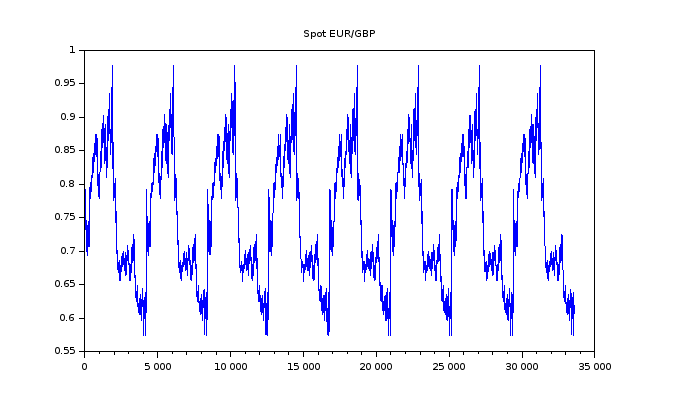
\includegraphics[scale=0.6]{Scilab-currencies.png}
\lstinputlisting[language=Octave, firstline=3, lastline=5]{../Perl/readCharges}
This is the graph of the EUR/GBP 

\section{Cash balance}
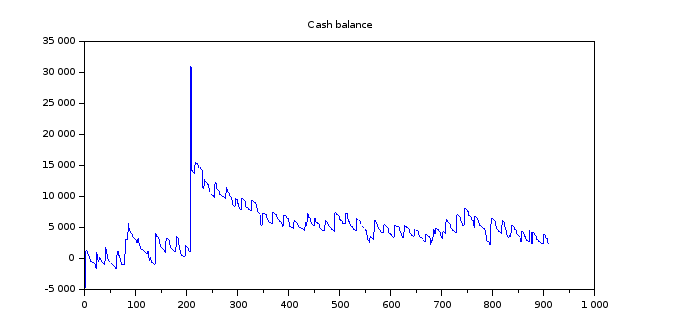
\includegraphics[scale=0.6]{Scilab-cashBalance.png}
\lstinputlisting[language=Octave, firstline=3, lastline=5]{../Perl/readCharges}
This is the graph of my EUR cashbalance 

\section{Stocks}
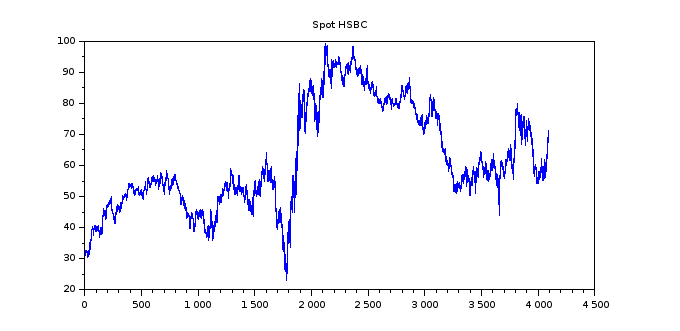
\includegraphics[scale=0.6]{Scilab-stocks.png}
\lstinputlisting[language=Octave, firstline=3, lastline=5]{../Perl/readCharges}
This is the graph of HSBC stock 

\subsubsection{Table}
Stocks table is available in the database ;-)
select * from stocks
%\begin{longtable}{|c|c|c|c|c|}
\hline
\multicolumn{5}{|c|}{Cashflows} \\
\hline
Category & Debit & Credit & PnL \\
\hline
Other & 0.0000001 & 0.0000001 & 0\\
\hline
Other & 104 & 0 & -104\\
\hline
Other & 13 & 0 & -13\\
\hline
Other & 10 & 0 & -10\\
\hline
Other & 190 & 0 & -190\\
\hline
Other & 8 & 0 & -8\\
\hline
Other & 16 & 0 & -16\\
\hline
Other & 4 & 0 & -4\\
\hline
Other & 6 & 0 & -6\\
\hline
Other & 14 & 0 & -14\\
\hline
 ... & ... & ... & ...\\
\hline
 Total & 112143.00006290044 & 117930.00006290042 & 5786.99999999999 \\
\hline
\end{longtable}

\subsubsection{Graph}
The graph is also available and produced by C++ under "legends"
\begin{bchart}[min=0,max=11214,step=3738,unit=k\texteuro]
\bcbar[label=Other]{0}\\
\smallskip
\bcbar[label=Other]{10}\\
\smallskip
\bcbar[label=Other]{1}\\
\smallskip
\bcbar[label=Other]{1}\\
\smallskip
\bcbar[label=Other]{19}\\
\smallskip
\bcbar[label=Other]{0}\\
\smallskip
\bcbar[label=Other]{1}\\
\smallskip
\bcbar[label=Other]{0}\\
\smallskip
\bcbar[label=Other]{0}\\
\smallskip
\bcbar[label=Other]{1}\\
\smallskip
\end{bchart}

\lstinputlisting[language=Octave, firstline=3, lastline=5]{../Perl/readCharges}
%\includepdf[pages={1}]{stockchart.pdf}

\end{document}

